
%% Copyright 2019-2024 Elsevier Ltd
%% 
%% This file is part of the 'CAS Bundle'.
%% --------------------------------------
%% 
%% It may be distributed under the conditions of the LaTeX Project Public
%% License, either version 1.3c of this license or (at your option) any
%% later version.  The latest version of this license is in
%%    http://www.latex-project.org/lppl.txt
%% and version 1.3c or later is part of all distributions of LaTeX
%% version 1999/12/01 or later.
%% 
%% The list of all files belonging to the 'CAS Bundle' is
%% given in the file `manifest.txt'.
%% 
%% Template article for cas-sc documentclass for
%% single column output.

\documentclass[a4paper,fleqn]{cas-sc}

% If the frontmatter runs over more than one page
% use the longmktitle option.

%\documentclass[a4paper,fleqn,longmktitle]{cas-sc}

\usepackage[numbers]{natbib}
%\usepackage[authoryear]{natbib}
%\usepackage[authoryear,longnamesfirst]{natbib}
\usepackage{graphicx}
\usepackage{booktabs}
\usepackage{array}
\usepackage{algorithm}
\usepackage{algpseudocode}
\usepackage{enumitem}   
\usepackage{tabularx}

%%%Author macros
\def\tsc#1{\csdef{#1}{\textsc{\lowercase{#1}}\xspace}}
\tsc{WGM}
\tsc{QE}
%%%

\begin{document}
\let\WriteBookmarks\relax
\def\floatpagepagefraction{1}
\def\textpagefraction{.001}

% Short title
\shorttitle{TE-Q-Transformer for Battery SOH Estimation}

% Short author
\shortauthors{ZA Lisan et~al.}

% Main title of the paper
\title[mode=title]{TE-Q-Transformer: A Temperature-Embedded Quantum Framework for Battery State-of-Health Estimation}

% First author
\author[1]{Zadid Al Lisan}[orcid=0009-0001-1801-051X]
\ead{lisan15-5426@diu.edu.bd}

\author[1]{Md. Sulyman Islam Sifat}[orcid=0009-0005-6377-8973]

\ead{sifat15-4004@diu.edu.bd}

\author[3]{M.S. Hossain Lipu}[orcid=0000-0001-9060-4454] % replace XXXX with correct last 4 digits
\ead{molla_lipu@uow.edu.au}


\author[2]{Nazakat Ali}[orcid=0000-0002-3875-812X] % replace XXXX with correct last 4 digits
\ead{nazakat.ali@se.abb.com}



\author[1]{Md Alamgir Kabir}[orcid=0000-0002-7136-6339]
\ead{kabir.cse@diu.edu.bd}
\cormark[1]
%\credit{Conceptualization, Project administration, Writing – review \& editing, Supervision}

\affiliation[1]{organization={Department of Computer Science and Engineering, Daffodil International University},
            city={Dhaka},
            country={Bangladesh}}

\affiliation[2]{organization={ABB},
    city={Vasteras},
    country={Sweden}}

\affiliation[3]{organization={School of Electrical, Computer and Telecommunications Engineering, University of Wollongong},
    city={New South Wales 2522},
    country={Australia}}

    
% Corresponding author text
\cortext[1]{Corresponding author}
% Footnote text
\fntext[1]{}

\begin{abstract}
% Accurate state of health (SOH) estimation is fundamental to the safe and efficient operation of lithium-ion batteries in electric vehicles and renewable energy systems. Although battery degradation is influenced by various operating conditions, temperature remains one of the most critical factors affecting battery ageing. However, most data-driven SOH estimation models treat temperature as a standard input feature rather than explicitly modeling its impact on degradation. Consequently, their ability to generalize across unseen battery cells operating under different thermal conditions remains limited. To address this limitation, we propose a temperature-embedded quantum transformer named TE-Q-Transformer, a physics-informed hybrid quantum-classical framework that integrates Arrhenius-based ageing physics into quantum feature. The model embeds trainable activation-energy parameters within a 4-qubit quantum circuit to capture temperature-dependent degradation, followed by a lightweight transformer encoder for SOH estimation. The proposed framework is evaluated on two public benchmarks, the NASA battery dataset and the CALCE battery dataset, using a fixed hybrid cross-cell held-out split for each. On NASA, TE-Q-Transformer achieves an RMSE of 0.031, MAE of 0.026, and $R^2$ score of 0.516 against five representative baselines. On CALCE, the same architecture achieves an RMSE of 0.0409, MAE of 0.0334, and $R^2$ score of 0.870, again outperforming five baselines. These findings suggest that integrating Arrhenius-based ageing physics into quantum feature learning improves cross-cell generalization and enables more reliable SOH estimation across varying operating temperatures.
Accurate state of health (SOH) estimation is fundamental to the safe and efficient operation of lithium-ion batteries in electric vehicles and renewable energy systems. Although battery degradation is influenced by various operating conditions, temperature remains one of the most critical factors affecting battery ageing. However, most data-driven SOH estimation models treat temperature as a standard input feature rather than explicitly modeling its impact on degradation. Consequently, their ability to generalize across unseen battery cells operating under different thermal conditions remains limited. To address this limitation, we propose a temperature-embedded quantum transformer, TE-Q-Transformer, a physics-informed hybrid quantum-classical framework that integrates Arrhenius-based ageing physics into quantum feature. The model embeds trainable activation-energy parameters within a 4-qubit quantum circuit to capture temperature-dependent degradation. The proposed framework is evaluated on two public benchmarks, NASA and CALCE battery dataset. On NASA, TEQ-Transformer achieves an RMSE of 0.031, MAE of 0.026, and $R^2$ score of 0.516 against five representative baselines. On CALCE, the same architecture achieves an RMSE of 0.0409, MAE of 0.0334, and $R^2$ score of 0.870, outperforming five baselines. These findings suggest that integrating Arrhenius-based ageing physics into quantum feature learning improves cross-cell generalization and enables more reliable SOH estimation across varying operating temperatures.
\end{abstract}

% Research highlights
% \begin{highlights}
% \item We propose TE-Q-Transformer, a hybrid quantum-classical model for battery SOH estimation.
% \item An Arrhenius-informed quantum gate embeds thermal ageing physics directly into the model.
% \item The model gives the best cross-battery accuracy on the non-linear NASA dataset.
% % \item A fair NASA benchmark with a multi-temperature cross-cell held-out split is reported against five baseline models. The model is further validated on the CALCE dataset.
% \item The model is further validated on the CALCE dataset, where it again achieves the lowest RMSE and MAE and the highest $R^2$ among six models.
% \end{highlights}

% Keywords
\begin{keywords}
Quantum machine learning \sep Battery state of health \sep Hybrid quantum-classical model \sep Transformer \sep Arrhenius temperature encoding
\end{keywords}

\maketitle

% Main text
% Main text
\section{Introduction}\label{sec:intro}

Lithium-ion batteries play a central role in electric transport and energy storage because of their high energy density, long cycle life, and falling cost \citep{ralls2023role}. Reliable battery operation depends on the Battery Management System (BMS), which monitors the factors such as voltage, current, temperature, and State of Charge (SoC) to keep each cell within safe limits \citep{ali2025comprehensive}. Over time, battery State of Health (SOH), defined as the ratio of remaining usable capacity to the rated capacity, declines through mechanisms such as solid-electrolyte interphase (SEI) growth, lithium plating, and active material loss \citep{li2025deep}. Accurate SOH estimation is therefore needed for safe operation, longer battery life, and better energy management.

Among the factors that influence this degradation process, temperature is one of the most important. Low temperature slows lithium-ion transport and increases the risk of lithium plating, while high temperature accelerates SEI growth and electrolyte breakdown \citep{kumar2024,asiri2025}. Battery ageing is therefore strongly linked to thermal conditions. Most data-driven models (e.g., \citep{liu2025multi}, \citep{li2025unified}, \citep{yang2025physics} and \citep{sun2025battery}), however, treat temperature as a normal input feature rather than as a physical driver of degradation. As a result, they often fail to capture the non-linear thermal effects that shape SOH trajectories. This limitation becomes more serious when models must generalize beyond the conditions seen during training. Different cells can follow different ageing patterns because of differences in manufacturing, chemistry, and usage history \citep{lu2024mechanisms}. Cross-battery evaluation is therefore difficult, and random train-test splits can overstate model performance \citep{sedlavrik2025advanced}. Together, these issues highlight the need for an SOH estimation framework that combines thermal ageing physics with robust generalization across unseen batteries.

Many studies have therefore turned to data-driven SOH methods on both laboratory and real-vehicle data. Such as Zhao et al. \citep{zhao2025capacity} fused a CNN-GRU model with Gaussian process regression and showed accurate capacity tracking on fleet data. Wang et al. \citep{wang2026lithium} validated their model on laboratory cells and a 260-vehicle real-world EV fleet. Moreover, Wen et al. \citep{wen2024lithium} used an interpretable boosting framework on pure electric vehicles and reported strong SOH accuracy under real charging behaviour. Furthermore, Liu et al. \citep{liu2025multi} proposed a multi-modal ResNet model on open-source field data and improved on common baselines such as SVR, random forest, GPR, and LSTM. Also, Sun et al. \citep{sun2025battery} applied a BO-XGBoost model with attention and also reached low estimation error. Together, these works show clear progress in learning from sequence data and large-scale vehicle records. However, most of them still feed temperature into the model in the same way as voltage and current. This limits their ability to represent Arrhenius-type thermal ageing \citep{gao2023effect}, which is one reason why performance can drop when models are tested on cells or operating conditions that differ from the training set. Since these classical models still struggle to represent the complex non-linear degradation mechanism, recent research has begun to explore hybrid quantum-classical learning as an alternative approach.

Hybrid quantum-classical models have been studied for battery health prediction with the aim of learning non-linear degradation patterns under limited data. For example, Soon and Soon \citep{soon2025hybrid} combined a quantum neural network with a GRU and obtained high correlation with measured SOH on NASA cells. Similarly, Mutua et al. \citep{mutua2025} used a variational quantum neural network on NASA batteries and slightly outperformed a classical LSTM baseline. In another approach, Liang et al. \citep{liang2025stochastic} proposed a quantum convolutional neural network with automated feature fusion and reported clear RMSE gains over CNN, MLP, and LSTM models. Moreover, Wang et al. \citep{wang2024lithium} used a variational quantum algorithm with a stacking strategy and kept SOH error low on laboratory cells. More recently, Wang and Kebede \citep{wang2026prediction} applied a QLSTM with transfer learning on CAN-bus charging data from 20 vehicles and further improved prediction accuracy. These results suggest that quantum components can add useful non-linearity to SOH modelling. However, temperature is still rarely encoded as a physical mechanism inside the quantum circuit. In most quantum models, temperature is either treated like other sensor channels or handled through classical preprocessing before standard angle encoding. Therefore, there remains a need for a hybrid model that embeds temperature-driven ageing physics directly into quantum representations while preserving temporal sequence modelling capability.

To address this gap, we propose Temperature-Embedded Quantum Transformer called TE-Q-Transformer, a hybrid model for SOH estimation from raw multi-channel battery sequences. First, temperature is mapped to a rotation angle through an Arrhenius-informed gate with trainable activation-energy linked to SEI growth and lithium plating. Besides, voltage, current, and normalized time are mapped to $\pi$-scaled rotations. Then, an expressive entangling circuit produces a quantum feature vector and is passed to a transformer encoder with CLS pooling and a small Multi-Layer Perceptron (MLP) head. The design keeps the overall pipeline lightweight relative to deep classical frameworks that is relevant for practical battery monitoring settings with limited compute resources.

% \citep{rahman2026}. 

The main contributions of this paper are as follows.
\begin{enumerate}[label=(\roman*)]
\item Model development: TE-Q-Transformer is proposed as a hybrid quantum-classical model in which an Arrhenius-informed temperature gate is incorporated, allowing thermal ageing effects to be embedded into the quantum state rather than treating temperature as a conventional feature. 
% for 
% for Li-ion battery SOH prediction by utilizing voltage, current, temperature, and time sequences.
% \item We introduce an Arrhenius-informed temperature gate that embeds thermal ageing effects into the quantum state instead of treating temperature as a normal feature.
\item Validation: A benchmark is presented on two public datasets, NASA and CALCE, using a hybrid cross-cell held-out protocol against classical and hybrid quantum-classical baselines.
\item Benchmarking and comparative analysis: The proposed framework demonstrates improvement on cross-battery generalization for Li-ion battery SOH prediction on both datasets. For reproduction of our proposed architecture, the codes are available online at \href{https://github.com/LisanHub/Te-Q-Transformer}{https://github.com/LisanHub/Te-Q-Transformer}.
% on the non-linear NASA dataset.
\end{enumerate}

The remainder of this paper is organized as follows. Section~\ref{sec:method} presents the methodology, including the NASA and CALCE datasets and preprocessing, the hybrid cross-cell held-out training protocols, the classical and hybrid quantum-classical baselines, and the proposed TE-Q-Transformer architecture with its Arrhenius-informed quantum embedding and Transformer stages. Section~\ref{sec:results} reports the experimental findings on the NASA benchmark, covering quantitative metrics against five baselines, cell-wise SOH trajectory analysis under the held-out thermal conditions, a component ablation of the proposed architecture, and an evidence-based analysis of the key claims, followed by a cross-dataset validation on CALCE. Section~\ref{sec:conclusion} concludes the paper and outlines directions for future work.

% \clearpage %%Remove this from your manuscript


\section{Methodology}\label{sec:method}

\begin{figure}
  \centering
    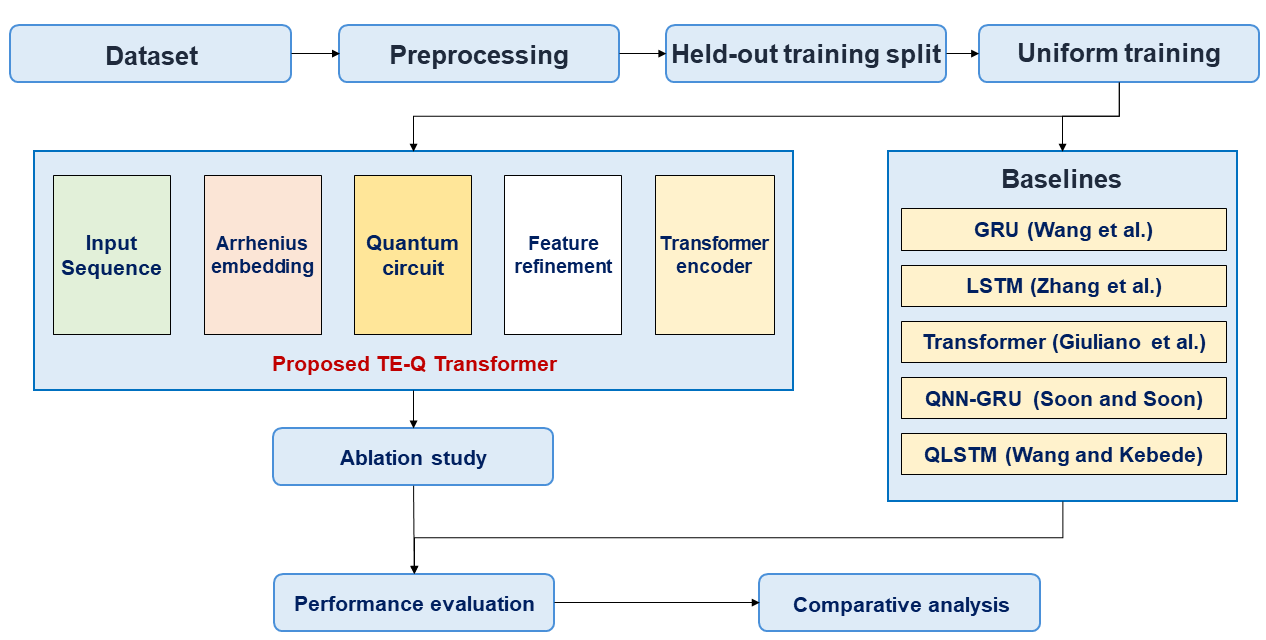
\includegraphics[width=\linewidth]{figs/teq_methodology.png}
    \caption{Overall workflow diagram }\label{methodology}
\end{figure}
This section describes the dataset, the training protocol, the baseline models, and the proposed TE-Q-Transformer framework. We pre-process the data and perform the experiment with a uniform training protocol across five baselines and our proposed model. We then conduct an ablation study before evaluating the performance along with comparative analysis. The overall workflow diagram is presented in Figure~\ref{methodology}. 

\subsection{Datasets and preprocessing}\label{sec:datasets}
To ensure that the proposed architecture is unbiased towards any specific dataset, we test TE-Q-Transformer on two publicly available datasets, NASA and CALCE.

The NASA battery dataset \cite{saha2007battery} is utilized as the primary benchmark since it has been adopted as a de facto standard for the evaluation of battery health estimation models \citep{komarsofla2026}. The dataset includes voltage, current and temperature readings at regular intervals during charge and discharge cycles. Since this study involves temperature embedding into quantum state, our NASA evaluation focuses on three thermally distinct cells: (i) B0018 at 24\,$^\circ$C, (ii) B0032 at 43\,$^\circ$C, and (iii) B0053 at 4\,$^\circ$C. This range from low to high ambient temperature supports our focus on temperature-aware SOH modelling.

As a second, independent benchmark, we use the CALCE battery dataset~\citep{w9rg-7173-25} from the Center for Advanced Life Cycle Engineering at the University of Maryland. Unlike NASA, the CALCE cells (CS2 series, lithium cobalt oxide prismatic cells) are cycled under a fixed ambient temperature and a constant-current constant-voltage protocol, so this dataset provides a cross-chemistry, cross-laboratory check on the generalization claims made on NASA rather than a further test of temperature-aware modelling. We use four CS2 cells for this benchmark: CS2\_35 and CS2\_36 form the full training set, CS2\_37 is split chronologically in the same way as B0053 on NASA, and CS2\_38 is reserved as a fully held-out test cell, with the same voltage, current, temperature, and normalized-time input channels as NASA.

For both datasets, SOH is defined per cell as the current measured capacity divided by that cell's first-cycle capacity. Each input window contains 512 time steps with four features: voltage, current, temperature, and normalized time. Only voltage, current, and normalized time are scaled with min-max normalization. The scaler is fitted on the training set only and then applied to the test set. Temperature is kept in raw degrees Celsius so that the Arrhenius gate receives physically meaningful values.

\subsection{Training protocol}\label{sec:training}
We apply a fixed hybrid multi-temperature cross-cell held-out protocol inspired by recent studies (e.g. \citep{sahoo2022transfer}, \citep{che2023increasing}, and \citep{kumar2026temperature}).
Training and testing are strictly separated by cell identity, while data from one cell are divided based on time.
The full training set utilizes all recorded data from cells B0005, B0006, B0007, B0029, B0030, and B0031. Cells B0018 and B0032 are reserved as full test cells and never appear during training. Cell B0053 is split chronologically: the first 70\% of cycles are used for training and the remaining 30\% for testing (B0053\_test). Chronological order is preserved in all windows.

The same cross-cell held-out logic is applied to CALCE. Cells CS2\_35 and CS2\_36 contribute all of their cycles to training, cell CS2\_38 is reserved as a full test cell and never appears during training, and cell CS2\_37 is split chronologically with the first 70\% of cycles used for training and the remaining 30\% for testing (CS2\_37\_test). As on NASA, the min-max scaler used for voltage, current, and normalized time is fit on the CALCE training cells only, and chronological order is preserved within every window.

All models are evaluated with the same windowing, preprocessing, split rules, and metrics on both datasets. We report Root Mean Squared Error (RMSE), Mean Absolute Error (MAE), and the coefficient of determination (R\textsuperscript{2}). Table~\ref{tbl1} summarizes the training, windowing, and common architecture settings shared by all models on the NASA benchmark; the CALCE benchmark reuses the same windowing, scaling, optimization, and architecture settings, with the cell-level split described above.

\begin{table}%[]
\caption{Training, windowing, and common architecture settings for NASA dataset.}\label{tbl1}
\begin{tabular*}{\tblwidth}{@{}LL@{}}
\toprule
Item & Setting \\
\midrule
\multicolumn{2}{l}{\textit{Data and windowing}} \\
Input features & Voltage, Current, Temperature, Time (normalized) \\
Sequence length & 512 time steps per window \\
SOH definition & Current capacity divided by first-cycle capacity (per cell) \\
Preprocessing & Min-max scaling for voltage, current, and time (fit on train only). Temperature in raw $^\circ$C \\
Split protocol & Hybrid multi-temperature cross-cell held-out split \\
Training set & B0005--B0007, B0029--B0031, first $70\%$ of B0053 \\
Test set & B0018, B0032, remaining $30\%$ of B0053 \\
Evaluation metrics & RMSE, MAE, R\textsuperscript{2} \\
\midrule
\multicolumn{2}{l}{\textit{Common architecture}} \\
Model dimension & $d_{\mathrm{model}}=64$ \\
Encoder depth & 1 layer \\
Dropout & 0 \\
Regression head & $\mathrm{Linear}(64,64)$ $\rightarrow$ GELU $\rightarrow$ $\mathrm{Dropout}$ $\rightarrow$ $\mathrm{Linear}(64,1)$ \\
\midrule
\multicolumn{2}{l}{\textit{Optimization and training}} \\
Optimizer & AdamW; learning rate $10^{-3}$; weight decay $5\times10^{-2}$ \\
Loss function & Mean squared error (MSE) \\
Learning-rate scheduler & ReduceLROnPlateau; factor $0.5$; patience $10$ \\
Gradient clipping & Maximum norm $1.0$ \\
Early stopping & Patience $20$ based on training loss \\
Training epochs & $80$ \\
Batch size & $8$ \\
\bottomrule
\end{tabular*}
\end{table}

\subsection{Baseline models}\label{sec:baselines}
We compare TE-Q-Transformer with five baselines from recent SOH estimation studies (i.e., \citep{wang2024state, zhang2023accurate, giuliano2025transformer, soon2025hybrid, wang2026prediction}). There are two types of baselines: deep learning sequence models and hybrid quantum-classical models. 

Three classical architectures that learn SOH directly from temporal sensor data comprise the deep learning group. The following are examples of these:  
\begin{enumerate}[label=(\roman*)]
  \item \textbf{Wang et al.~\citep{wang2024state}:} This study combined empirical mode decomposition with Random Forest and GRU networks for battery health estimation.  They used charge and discharge voltage curves to extract time-based features, decomposed capacity data into smoother components, and used various models to the fluctuating and steady parts. This design enhanced the accuracy of the data and decreased the computation time for NASA battery information. We take this approach as the GRU baseline.
  \item \textbf{Zhang et al.~\citep{zhang2023accurate}:} The authors utilized a LSTM network that that monitors the battery capacity degradation with time. The capacity was used as the primary health indicator and history was fed into the model in the form of sequences of ages. Tests on NASA batteries showed that the approach can predict remaining capacity and remaining useful life reliably. We consider this method as our LSTM baseline.
  \item \textbf{Giuliano et al.~\citep{giuliano2025transformer}:} They proposed a Transformer that uses attention to capture long-term ageing trends across battery cycles. They studied transfer from one battery type on the NASA dataset to another chemistry on the Oxford dataset. After fine-tuning, the Transformer improved accuracy and outperformed models trained only on the target data. This architecture is used as our Transformer baseline.
\end{enumerate}

Furthermore, the hybrid quantum-classical group combines quantum circuits with classical sequence learning. These are given below:
\begin{enumerate}[label=(\roman*)]
  \item \textbf{Soon and Soon \citep{soon2025hybrid}:} The authors paired a quantum neural network with a classical GRU forming QNN-GRU. They used three easy-to-measure discharge features as inputs. The hybrid model achieved lower prediction error than several standard machine learning methods on NASA batteries. This design corresponds to our QNN-GRU baseline.
  \item \textbf{Wang and Kebede \citep{wang2026prediction}:} They developed a quantum-enhanced LSTM (QLSTM) with shared embedding layers and transfer learning for electric-vehicle battery pack health estimation. 
  % The method was designed for partial real-world charging data collected from multiple vehicles over many months. 
  % Training on several packs together gave better accuracy than training on a single pack, with very low prediction error. 
  This approach is implemented as our QLSTM baseline.
\end{enumerate}

Table~\ref{tab:nasa_baseline_config} reports the model-specific configurations of these five baselines, including feature projection, sequence encoder, attention, feed-forward width, quantum circuit, positional encoding, and sequence representation. The same five configurations, without any dataset-specific tuning, are reused for the CALCE benchmark in Section~\ref{sec:calce}, so that differences in accuracy between the two datasets reflect the data itself rather than a change in baseline design.

\begin{table*}[t]
\centering
\caption{Model-specific configurations of the baseline models evaluated on the NASA battery dataset. Shared architecture, optimization, and data-processing settings are listed in Table~\ref{tbl1}.}
\label{tab:nasa_baseline_config}
\footnotesize
\setlength{\tabcolsep}{4pt}
\renewcommand{\arraystretch}{1.18}

\begin{tabular}{>{\raggedright\arraybackslash}p{0.16\textwidth}
                >{\centering\arraybackslash}p{0.16\textwidth}
                >{\centering\arraybackslash}p{0.16\textwidth}
                >{\centering\arraybackslash}p{0.16\textwidth}
                >{\centering\arraybackslash}p{0.16\textwidth}
                >{\centering\arraybackslash}p{0.16\textwidth}}
\toprule
\textbf{Configuration} &
Wang et al.~\newline\citep{wang2024state} &
Zhang et al.~\newline\citep{zhang2023accurate} &
Giuliano et al.~\newline\citep{giuliano2025transformer} &
Soon and Soon\newline\citep{soon2025hybrid} &
Wang and Kebede\newline\citep{wang2026prediction} \\
\midrule

Feature projection
& $\mathrm{Linear}(4,64)$
& $\mathrm{Linear}(4,64)$
& $\mathrm{Linear}(4,64)$
& $\mathrm{Linear}(4,4)$ $\rightarrow$ QNN $\rightarrow$ $\mathrm{Linear}(4,64)$
& $\mathrm{Linear}(4,4)$ $\rightarrow$ QNN $\rightarrow$ $\mathrm{Linear}(4,64)$ \\

Sequence encoder
& GRU
& LSTM
& Transformer Encoder
& GRU
& LSTM \\

Attention mechanism
& None
& None
& 4 attention heads
& None
& None \\

Feed-forward dimension
& --
& --
& $256$
& --
& -- \\

Quantum circuit
& --
& --
& --
& 4 qubits, 2 layers$^{\mathrm{a}}$
& 4 qubits, 2 layers$^{\mathrm{a}}$ \\

Positional encoding
& --
& --
& Sinusoidal
& --
& -- \\

Sequence representation
& Last hidden state
& Last hidden state
& Last token
& Last hidden state
& Last hidden state \\

\bottomrule
\end{tabular}

\vspace{3pt}
\begin{minipage}{0.98\textwidth}
\footnotesize
\textit{Note:}
$^{\mathrm{a}}$ The quantum circuit uses Y-axis AngleEmbedding, 
BasicEntanglerLayers, and Pauli-$Z$ expectation measurements implemented
with PennyLane \texttt{default.qubit} on CPU. The sinusoidal positional
encoding uses a maximum sequence length of $512$.
\end{minipage}

\end{table*}



\subsection{Proposed TE-Q-Transformer architecture}\label{sec:architecture}
The proposed model, TE-Q-Transformer, predicts battery state of health from sensor data using a five-stage pipeline. The model embeds known battery degradation physics directly into its input representation using a quantum circuit, then processes the resulting features over time with a transformer encoder to capture long-range temporal patt+erns. Figure~\ref{fig1} shows the full pipeline of the proposed model with five phases.

\begin{figure}
  \centering
    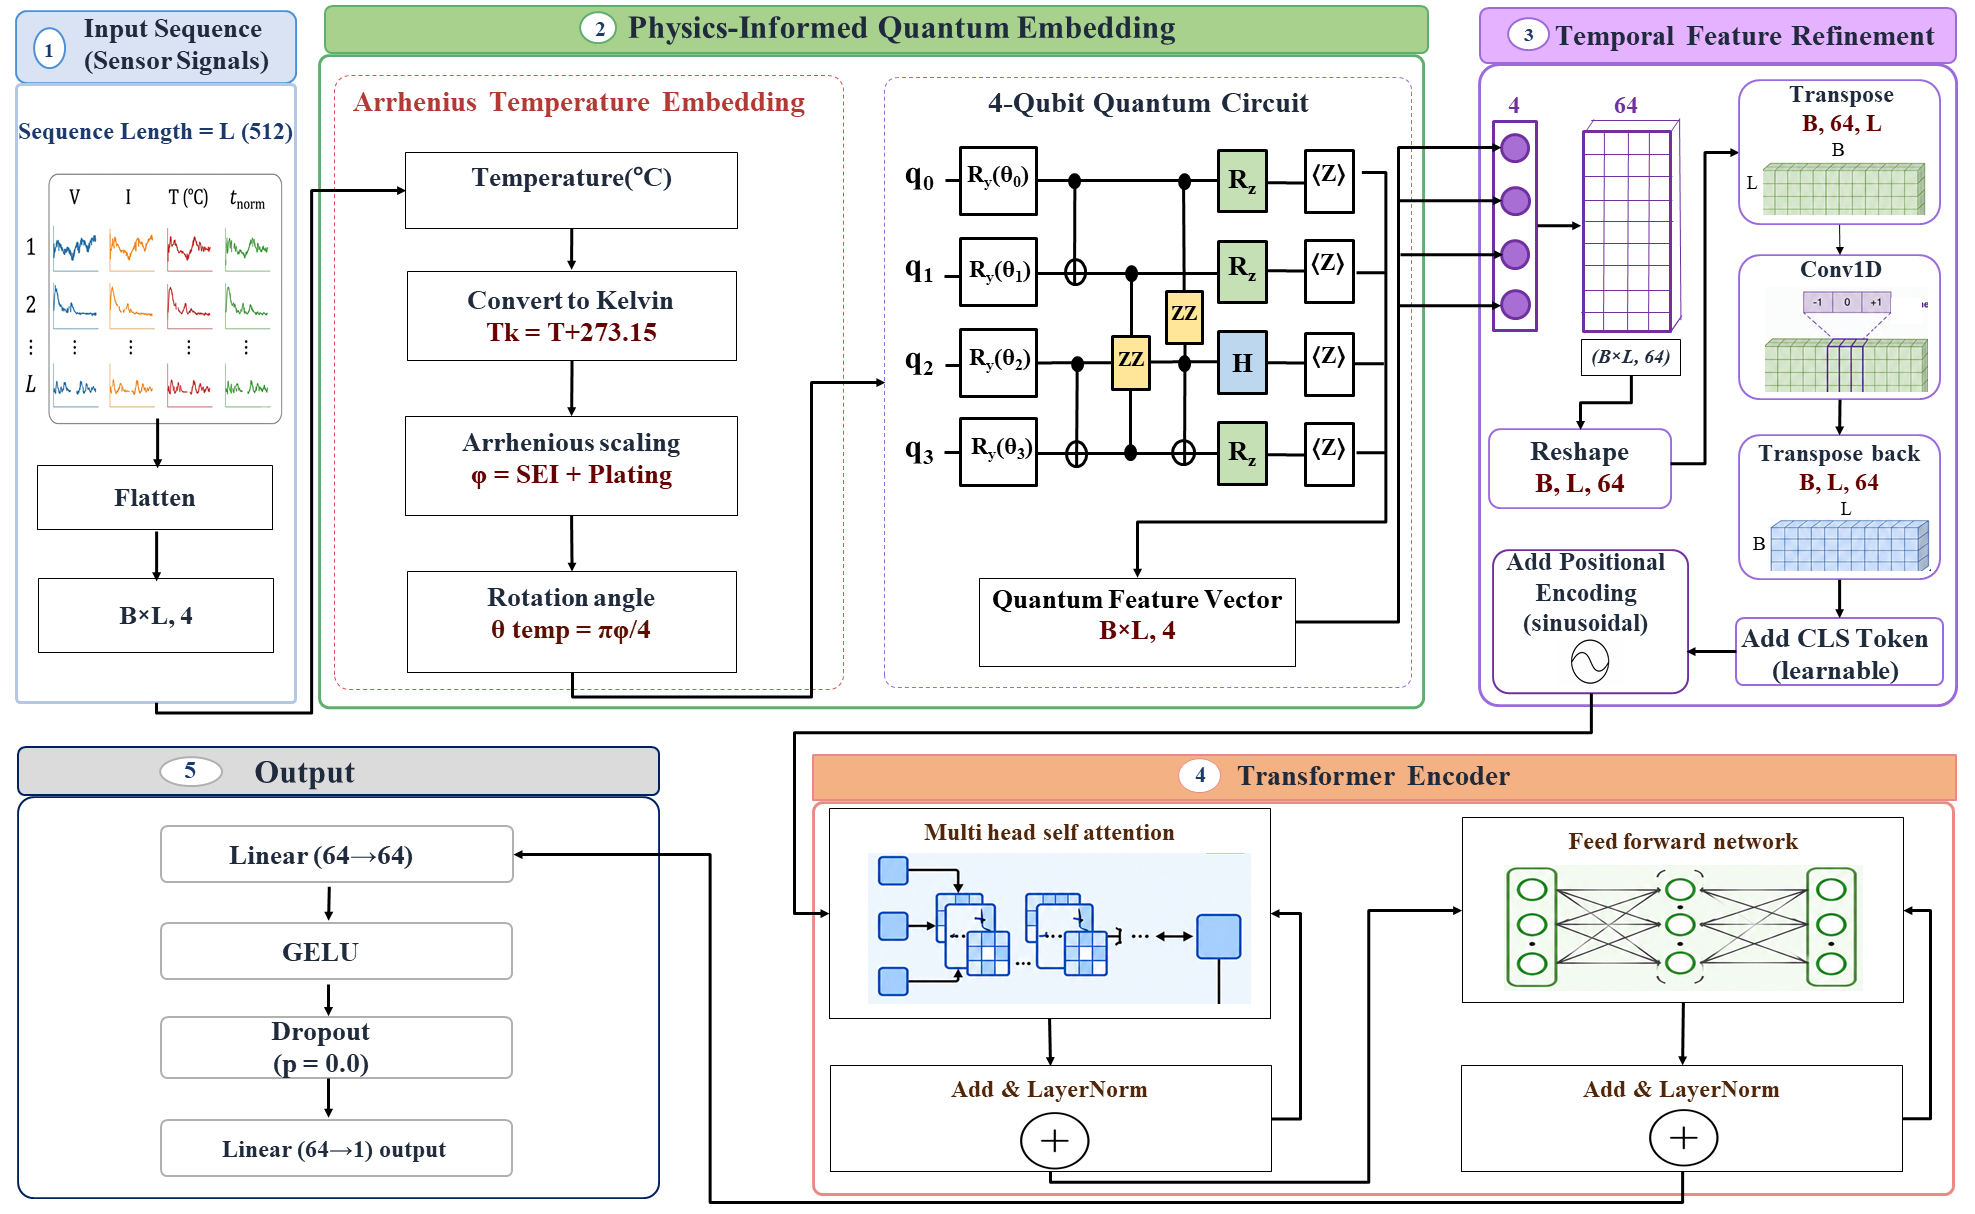
\includegraphics[width=\linewidth]{figs/teq_architecture.png}
    \caption{TE-Q-Transformer architecture: (1) input sensor sequence, (2) physics-informed quantum embedding with Arrhenius temperature gate, (3) temporal feature refinement, (4) Transformer encoder, and (5) SOH output head.}\label{fig1}
\end{figure}

\subsubsection{Phase 1: Input sensor sequence} The model receives a batch of input windows with shape $(B, L, 4)$, where $B$ is the batch size, $L=512$ is the sequence length, and the four features are voltage $V$, current $I$, temperature $T$ in degrees Celsius, and normalized time $t_{\mathrm{norm}}$. Temperature is kept in raw degrees Celsius so that the Arrhenius gate can use physical thermal values. The other three features are min-max scaled with a scaler fitted on the training set only to avoid data leakage. Finally, the tensor is then flattened to $(B \cdot L, 4)$ shape so that each time step can be processed independently by the quantum layer.

\subsubsection{Phase 2: Physics-informed quantum embedding with Arrhenius temperature gate}
The second phase converts each time-step reading into a small quantum feature vector. Instead of feeding temperature into the circuit as an ordinary scaled input, the model first uses well-known battery ageing physics to decide how strongly temperature should influence the quantum state. That idea is implemented in two consecutive layers: an Arrhenius temperature layer and a four-qubit quantum circuit. The Arrhenius layer focuses on two temperature-sensitive ageing processes that matter for lithium-ion cells. Solid electrolyte interphase (SEI) growth is one common source of capacity fade, and lithium plating becomes more relevant under cold operating conditions. The network learns two activation-energy parameters, $E_{a,\mathrm{sei}}$ and $E_{a,\mathrm{pl}}$, so that the embedding can adapt to how strongly each process should respond to temperature during training. Before those factors are computed, the measured temperature $T$ in degrees Celsius is converted to an absolute temperature $T_K$ in Kelvin by Eq.~\eqref{eq:kelvin}. It keeps the thermal input in physical units and avoids non-physical Kelvin values at the lower end.
\begin{equation}
T_K = \max(T + 273.15,\, 1). \quad \cite{waldmann2014temperature}
\label{eq:kelvin}
\end{equation}
A reference temperature $T_{\mathrm{ref}} = 298.15$\,K and the gas constant $R = 8.314$\,J\,mol$^{-1}$\,K$^{-1}$ are used in the Arrhenius terms below. The SEI-related thermal factor $\phi_{\mathrm{sei}}$ is demonstrated in Eq.~\eqref{eq:arrhenius-sei}. It increases or decreases the SEI contribution relative to room temperature, using $T_K$ from Eq.~\eqref{eq:kelvin}. 
\begin{equation}
\phi_{\mathrm{sei}} = \exp\!\left(\frac{E_{a,\mathrm{sei}} \cdot 10^{4}}{R}\left(\frac{1}{T_{\mathrm{ref}}} - \frac{1}{T_K}\right)\right). \quad \cite{kucinskis2022arrhenius}
\label{eq:arrhenius-sei}
\end{equation}
A separate Arrhenius term $\phi_{\mathrm{pl}}$ models lithium plating with the exponent arranged so that cold-temperature behaviour can be learned independently of SEI by Eq.~\eqref{eq:arrhenius-pl}.
\begin{equation}
\phi_{\mathrm{pl}} = \exp\!\left(\frac{E_{a,\mathrm{pl}} \cdot 10^{4}}{R}\left(\frac{1}{T_K} - \frac{1}{T_{\mathrm{ref}}}\right)\right). \quad \cite{yang2018understanding}
\label{eq:arrhenius-pl}
\end{equation}
Eq.~\eqref{eq:arrhenius-sei} works together with Eq.~\eqref{eq:arrhenius-pl} to form a combined thermal signal. That signal is turned into the temperature rotation angle $\theta_T$ by Eq.~\eqref{eq:theta-temp}.
\begin{equation}
\theta_T = \frac{\pi}{4}\left(\phi_{\mathrm{sei}} + \phi_{\mathrm{pl}}\right). \quad \cite{gao2017efficient}
\label{eq:theta-temp}
\end{equation}
Eq.~\eqref{eq:theta-temp} therefore links measured temperature to the quantum embedding through degradation physics rather than a fixed scaling rule. 


The four-qubit circuit is the second part of this stage. Voltage, current, and normalized time are already scaled to $[0,1]$; each channel is mapped to its own rotation angle on one qubit, while $\theta_T$ from Eq.~\eqref{eq:theta-temp} drives the temperature qubit. The voltage rotation angle $\theta_V$ is defined in Eq.~\eqref{eq:theta-v}.
\begin{equation}
\theta_V = \pi V. \quad \cite{hirai2024practical}
\label{eq:theta-v}
\end{equation}
Eq.~\eqref{eq:theta-v} maps the normalized voltage to a rotation in $[0,\pi]$. The current and time channels use the same linear mapping to angles $\theta_I$ and $\theta_t$ in Eq.~\eqref{eq:theta-i-t}.
\begin{equation}
\theta_I = \pi I, \qquad \theta_t = \pi t_{\mathrm{norm}}. \quad \cite{ovalle2023quantum}
\label{eq:theta-i-t}
\end{equation}
Eq.~\eqref{eq:theta-i-t} supplies the remaining input angles together with Eq.~\eqref{eq:theta-v} and Eq.~\eqref{eq:theta-temp}. Each angle is applied as an $R_y$ rotation on qubits $q_0$--$q_3$, which together form the encoding unitary $U_{\mathrm{enc}}$. The qubits are then mixed through a rich entangling unitary $U_{\mathrm{rich}}$ ($R_z$ gates, CNOTs, neighbouring Ising $ZZ$ couplings, Toffoli gates, Hadamard gates, and a closing $R_z$). Starting from the four-qubit ground state $\lvert 0\rangle^{\otimes 4}$, the resulting quantum state $\lvert\psi\rangle$ is given by Eq.~\eqref{eq:psi}.
\begin{equation}
\lvert\psi\rangle
=
U_{\mathrm{rich}}\,
U_{\mathrm{enc}}(\theta_V,\theta_I,\theta_t,\theta_T)\,
\lvert 0\rangle^{\otimes 4}.
\label{eq:psi}
\end{equation}
Eq.~\eqref{eq:psi} applies the angle embedding and the rich entangler to the four-qubit ground state. The circuit is simulated in PennyLane and trained end to end with backpropagation. Measuring the Pauli-$Z$ operators $Z_{0}$, $Z_{1}$, $Z_{2}$, and $Z_{3}$ on the four qubits yields the feature vector $\mathbf{q}$ in Eq.~\eqref{eq:pauli-z}.
\begin{equation}
\mathbf{q}
=
\bigl[
\langle\psi\rvert Z_{0}\lvert\psi\rangle,\,
\langle\psi\rvert Z_{1}\lvert\psi\rangle,\,
\langle\psi\rvert Z_{2}\lvert\psi\rangle,\,
\langle\psi\rvert Z_{3}\lvert\psi\rangle
\bigr]^{\top}.
\label{eq:pauli-z}
\end{equation}
Eq.~\eqref{eq:pauli-z} produces a four-dimensional representation for that time step, with overall output shape $(B \cdot L, 4)$ after processing the flattened batch. Algorithm~\ref{alg:quantum} summarizes the Arrhenius layer and the circuit in order.

\begin{algorithm}[t]
\caption{Physics-informed quantum embedding at one time step (Arrhenius layer and 4-qubit circuit)}
\label{alg:quantum}
\begin{algorithmic}[1]
\Require Scaled $V, I, t_{\mathrm{norm}} \in [0,1]$, raw temperature $T$ (\,$^\circ$C), trainable $E_{a,\mathrm{sei}}$, $E_{a,\mathrm{pl}}$
\Ensure Quantum feature vector $\mathbf{q} \in \mathbb{R}^{4}$
\State Compute $T_K$ from Eq.~\eqref{eq:kelvin}
\State Compute $\phi_{\mathrm{sei}}$ and $\phi_{\mathrm{pl}}$ from Eqs.~\eqref{eq:arrhenius-sei} and~\eqref{eq:arrhenius-pl}
\State Compute $\theta_T$ from Eq.~\eqref{eq:theta-temp}
\State Compute $\theta_V$, $\theta_I$, $\theta_t$ from Eqs.~\eqref{eq:theta-v} and~\eqref{eq:theta-i-t}
\State Apply $R_y(\theta_V)$, $R_y(\theta_I)$, $R_y(\theta_t)$, $R_y(\theta_T)$ on qubits $q_0$--$q_3$
\State Apply rich entangler: $R_z$, CNOT, Ising $ZZ$, Toffoli, Hadamard, $R_z$
\State Measure $\langle Z \rangle$ on each qubit and return $\mathbf{q}$ from Eq.~\eqref{eq:pauli-z}
\end{algorithmic}
\end{algorithm}


\subsubsection{Phase 3: Temporal feature refinement}
The third phase of the proposed model prepares the quantum features for sequence modeling. At each time step $\ell$, the four-dimensional quantum output $\mathbf{q}_{\ell}$ is not yet rich enough to support long-range learning on its own, so the model first projects it into a wider latent space and then smooths the result along the time axis. A linear layer with weight matrix $W_{p}$ and bias $\mathbf{b}_{p}$ expands the feature size from 4 to 64, as shown in Eq.~\eqref{eq:proj}.
\begin{equation}
\mathbf{h}_{\ell} = W_{p}\,\mathbf{q}_{\ell} + \mathbf{b}_{p}, \qquad W_{p}\in\mathbb{R}^{64\times 4}.
\label{eq:proj}
\end{equation}
Eq.~\eqref{eq:proj} maps each quantum vector into a projected token $\mathbf{h}_{\ell}$ in the Transformer latent space, and the sequence is reorganized back into batch form so that neighbouring time steps can be processed together. Then a one-dimensional convolution is performed with a small kernel that filters out the short-term variability in the signal without destroying the general trend of degradation. This step helps the model capture local temporal patterns before the global attention stage. To summarize the full window, a learnable CLS token is added at the start of the sequence, and sinusoidal positional encoding is applied so that the model knows the order of cycles within the 512-step input.

\subsubsection{Phase 4: Transformer encoder}
Building on this representation, the fourth stage uses a Transformer encoder to relate information across the whole sequence. Self-attention allows each time step, and the CLS token, to draw context from the rest of the window. For query, key, and value matrices $Q$, $K$, and $V$, and with $d_{k}$ denoting the per-head key dimension, scaled dot-product attention is defined in Eq.~\eqref{eq:attn}.
\begin{equation}
\mathrm{Attention}(Q,K,V)
=
\mathrm{softmax}\!\left(\frac{QK^{\top}}{\sqrt{d_{k}}}\right)V. \quad \cite{vaswani2017}
\label{eq:attn}
\end{equation}
Eq.~\eqref{eq:attn} links early and late parts of the degradation trajectory instead of relying only on local convolutions. The encoder uses three stacked layers with multi-head attention and feed-forward blocks, which is enough to model long-range dependencies in the NASA windows while keeping the network compact.

\subsubsection{Phase 5: SOH output head}
The final stage turns the encoded sequence into a single SOH value for each input window. The model reads the CLS token after the Transformer encoder, because that token is trained to aggregate information from the full sequence. The CLS representation $\mathbf{z}_{\mathrm{cls}}$ is passed through a small regression head with two linear layers, weight matrices $W_{1}$ and $W_{2}$, biases $\mathbf{b}_{1}$ and $\mathbf{b}_{2}$, and a GELU activation, as given in Eq.~\eqref{eq:head}.
\begin{equation}
\hat{y}
=
W_{2}\,\mathrm{GELU}(W_{1}\mathbf{z}_{\mathrm{cls}}+\mathbf{b}_{1})+\mathbf{b}_{2}.
\label{eq:head}
\end{equation}
Eq.~\eqref{eq:head} produces one scalar output $\hat{y}$. This value is the predicted SOH for the corresponding battery window.

% , which completes the forward path shown in Figure~\ref{fig1}.


% \clearpage

\section{Results and Discussion}
\label{sec:results}
We first present the test-set metrics for five baselines with our proposed framework. Next, we examine the predicted SOH curves under the three held-out conditions. We then report a component ablation of TE-Q-Transformer and discuss the combined findings. Section~\ref{sec:calce} closes the section with a cross-dataset validation on CALCE, using the same models and protocol.
% \subsection{NASA dataset results}
% \label{sec:nasa}

We present the results of RMSE, MAE, and R\textsuperscript{2} on the full test split (cells B0018 and B0032, and the last 30\% of cycles from B0053) in Table~\ref{tbl5}.
% Table~\ref{tbl5} lists RMSE, MAE, and R\textsuperscript{2} on the full test split: cells B0018 and B0032, plus the last 30\% of cycles from B0053. Every model uses the same 512-step windows, preprocessing, and metrics defined in Section~\ref{sec:method}.
\begin{table}%[]
\caption{Model performance on the NASA dataset. Lower RMSE and MAE, and higher R\textsuperscript{2} are better.}\label{tbl5}
\begin{tabular*}{\tblwidth}{@{}LLLL@{}}
\toprule
Model & RMSE & MAE & R\textsuperscript{2} \\
\midrule
Wang et al.~\citep{wang2024state} (GRU) & 0.0476 & 0.0412 & $-$0.6906 \\
Zhang et al.~\citep{zhang2023accurate} (LSTM) & 0.0409 & 0.0355 & 0.0010 \\
Giuliano et al.~\citep{giuliano2025transformer} (Transformer) & 0.0475 & 0.0411 & $-$0.3277 \\
Soon and Soon \citep{soon2025hybrid} (QNN-GRU) & 0.0339 & 0.0288 & $-$0.5235 \\
Wang and Kebede \citep{wang2026prediction} (QLSTM) & 0.0416 & 0.0368 & $-$0.1778 \\
Proposed (TE-Q-Transformer) & \textbf{0.0312} & \textbf{0.0257} & \textbf{0.5164} \\
\bottomrule
\end{tabular*}
\end{table}
The TE-Q-Transformer achieves the lowest RMSE (0.0312) and MAE (0.0257). It also obtains a positive R\textsuperscript{2} of (0.5164), indicating its ability to explain variations in the true SOH values. 
% and explaining the variation in true SOH.
% The proposed model shows better performance by demonstrating positive R\textsuperscript{2} of (0.5164) and explaining the variation in true SOH.
% on this split
% so its predictions explain part of the variation in true SOH on this split. 
The GRU, Transformer, QNN-GRU, and QLSTM models produce negative R\textsuperscript{2}, illustrating that they perform worse than baseline model that predicts the average SOH for every input window. Moreover, 
% . On this metric, their errors are larger than those from a naive predictor that outputs the same average SOH for every window. 
the LSTM achieves near zero  R\textsuperscript{2} (0.0010), showing the performance close to the baseline. Among the baseline models,  QNN-GRU gains lower RMSE and MAE than other classical models. However, its R\textsuperscript{2} remains negative value. 

% \subsection{Qualitative trajectory analysis}\label{sec:qualitative}
\subsection{Cell-wise result analysis}
\label{sec:qualitative}

\begin{figure}%[]
  \centering
    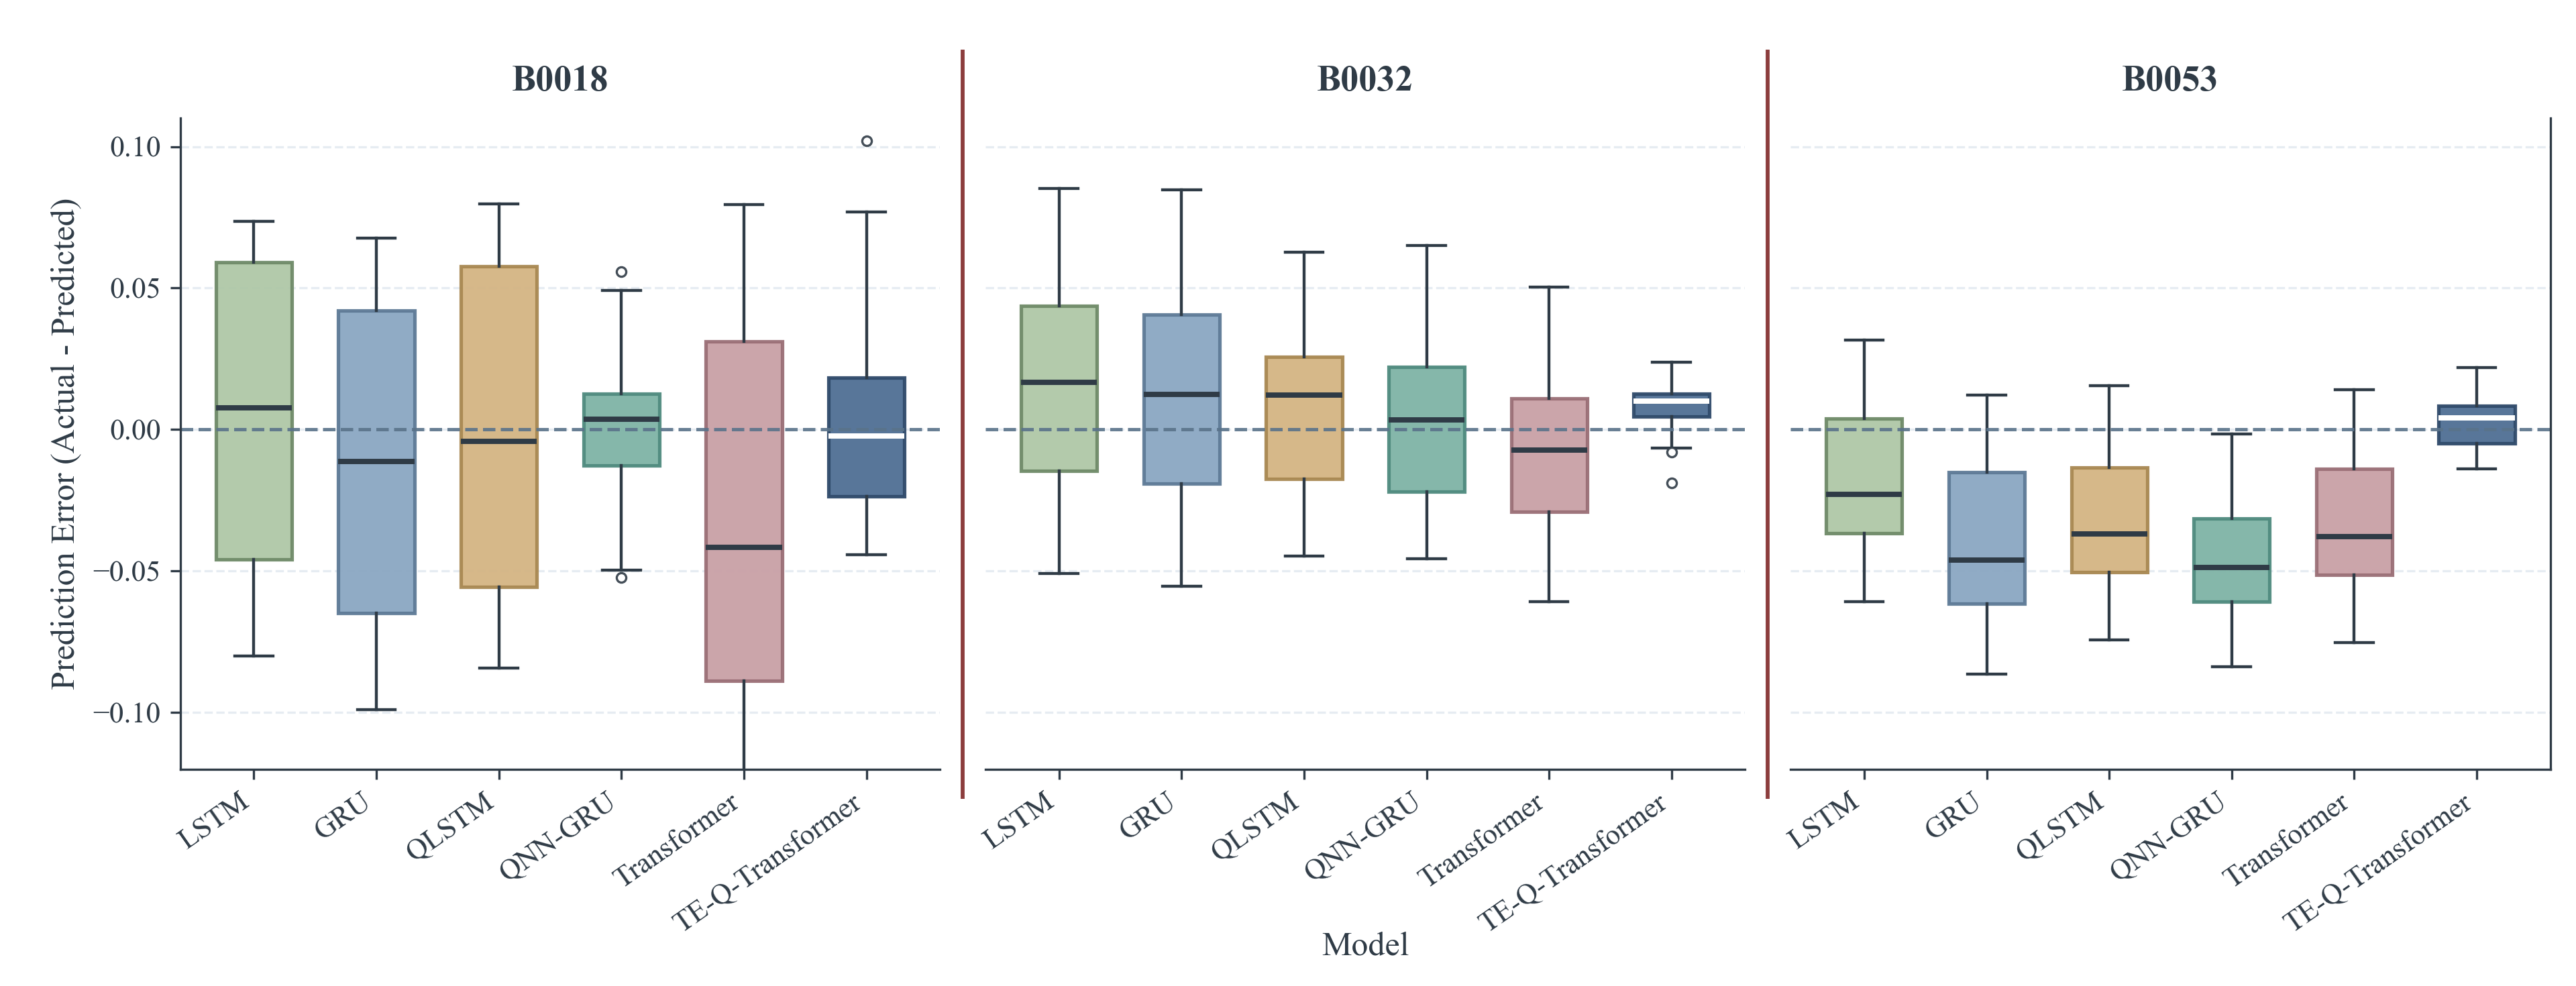
\includegraphics[width=\linewidth]{figs/error.png}
    \caption{Prediction error box plots for NASA test cells B0018, B0032, B0053 using the six models. The dashed line represents a zero error; the box represents the interquartile range, and the median is represented by the center line. B0053 uses the held-out late-life test tail.}\label{fig:nasa_error_boxplot_cells}
\end{figure}

\begin{figure}%[]
  \centering
    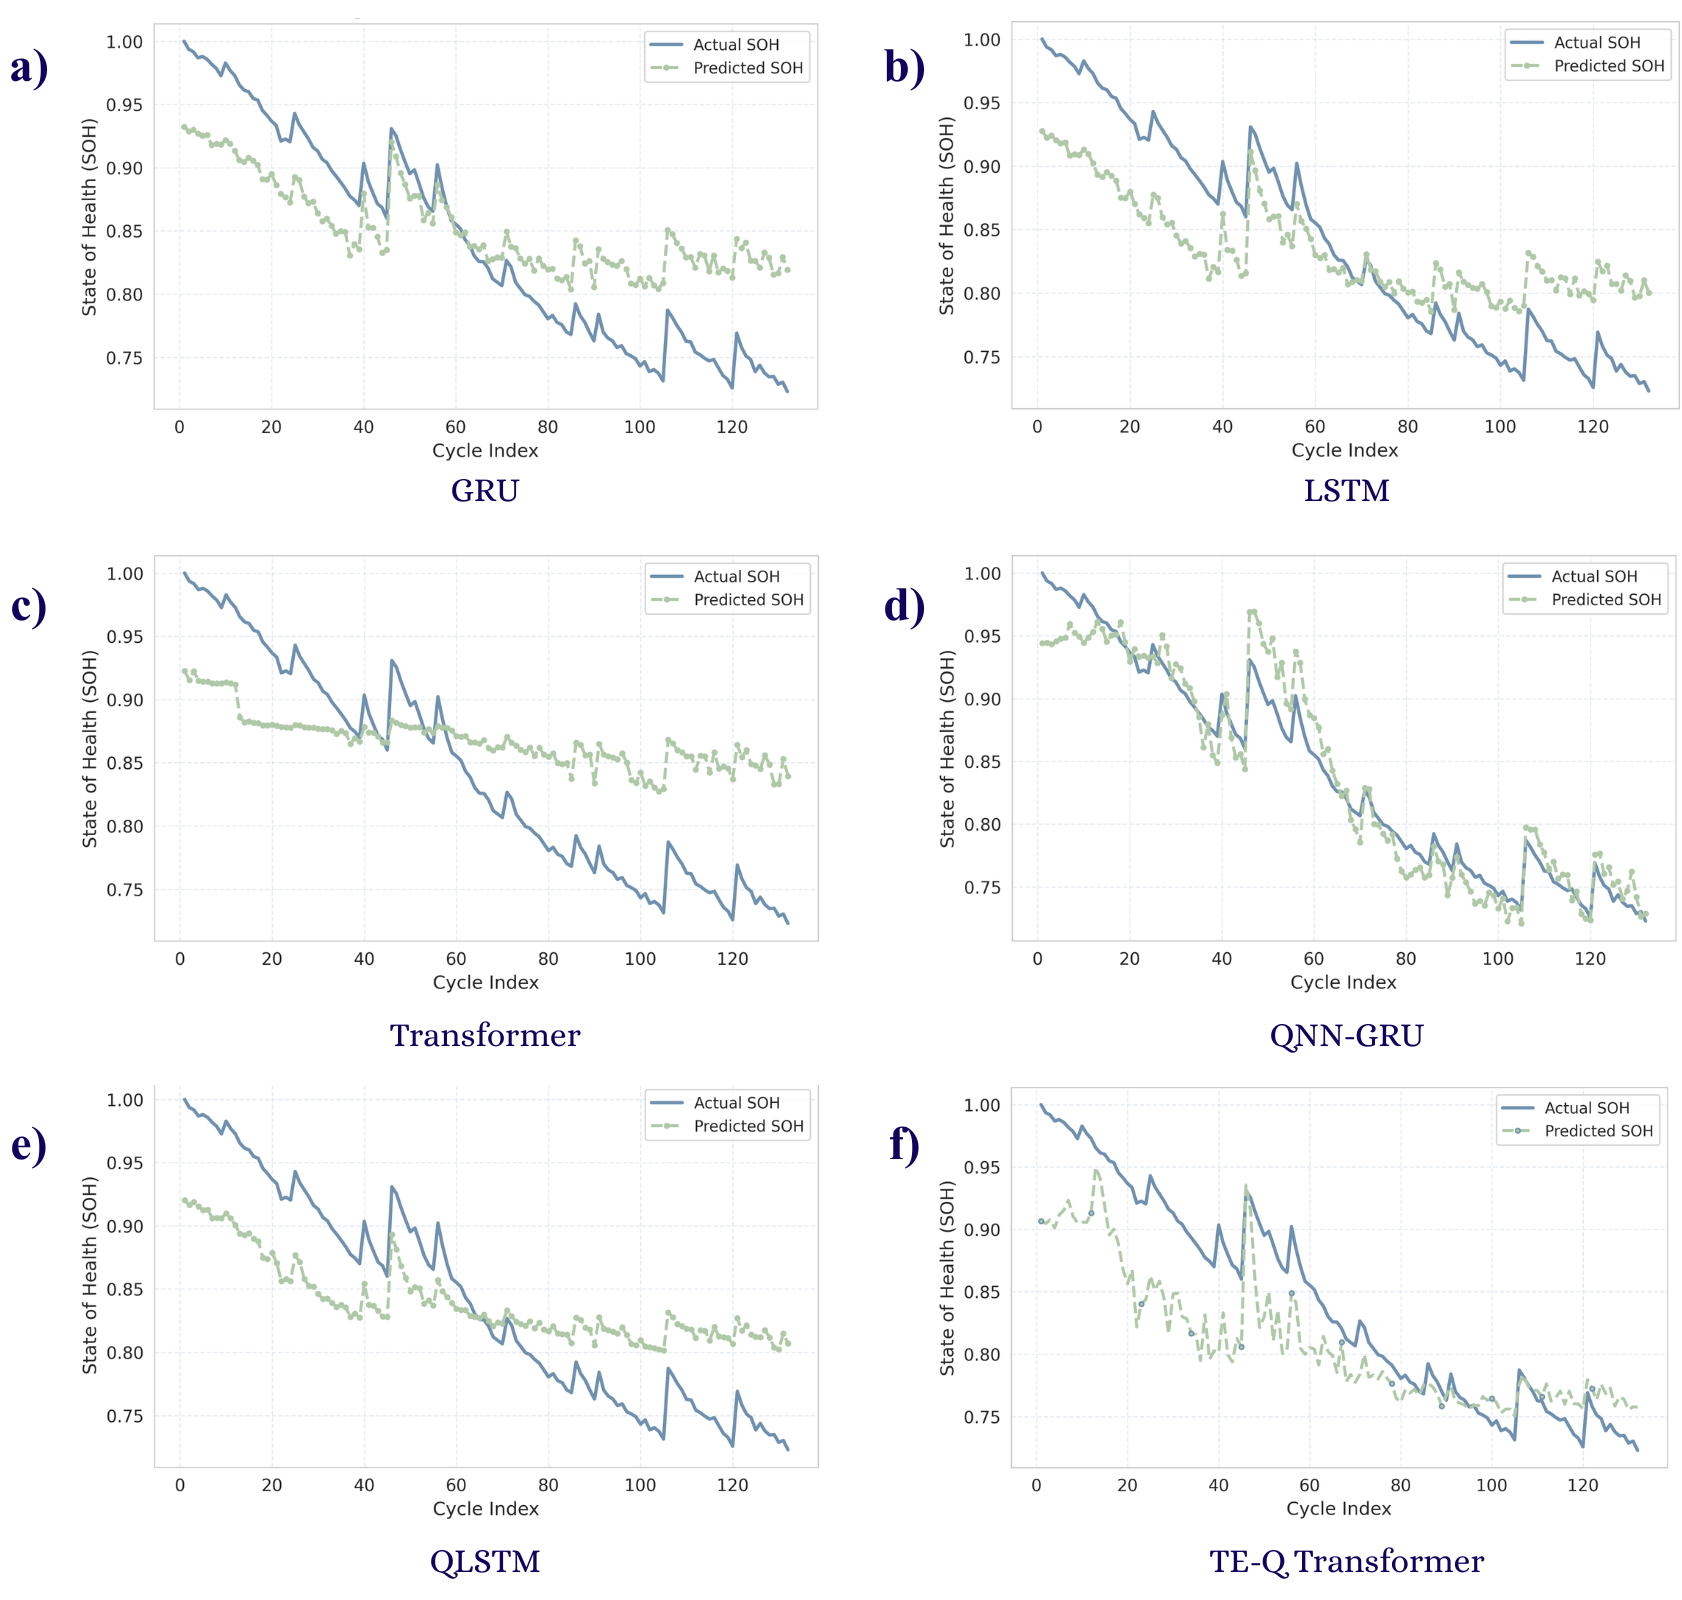
\includegraphics[width=\linewidth]{figs/NASA-b0018.png}
    \caption{Predicted versus actual SOH trajectories for held-out NASA test cell B0018 (24\,$^\circ$C). The TE-Q-Transformer follows the long degradation trend; LSTM collapses to a near-constant prediction.}\label{fig3}
\end{figure}
Regarding held-out cell B0018 at 24$^\circ$C, Figure~\ref{fig3} presents the results, which reveal a somewhat irregular decrease in the SOH from cycle to cycle. However, the baseline models do not follow these variations and tend to make relatively stable or nearly constant predictions instead. QNN-GRU (i.e., Figure~\ref{fig3}d)) gets closer to predicting the SOH, and the TE-Q-Transformer (i.e., Figure~\ref{fig3}f)) also captures the main variations, although with larger deviations at some cycles. The corresponding error distributions in Figure~\ref{fig:nasa_error_boxplot_cells} (left) show a wide spread for most models in this cell, with GRU and Transformer medians below the zero-error line and a more concise QNN-GRU box near zero. TE-Q-Transformer similarly keeps its median close to zero while remaining comparatively solid amid the high variance of B0018. This is reflected in the quantitative results: the TE-Q-Transformer achieves an RMSE of 0.0271, MAE of 0.0223, and $R^2$ of 0.8935, substantially improving over GRU (RMSE: 0.0535, $R^2$: 0.5866), LSTM (RMSE: 0.0504, $R^2$: 0.6327), and Transformer (RMSE: 0.0703, $R^2$: 0.2849). However, QNN-GRU performs slightly better on this cell, with an RMSE of 0.0208, MAE of 0.0166, and $R^2$ of 0.9375. Thus, the proposed model shows strong tracking ability on room temperature (B0018), although QNN-GRU provides the closest overall fit for this particular cell.

Figure~\ref{fig4} shows the results for held-out cell B0032 at 43$^\circ$C. In this case, the actual SOH decreases more rapidly during the middle part of the cell's life. Most baseline models either remain too high or fail to follow this overall decline, whereas the TE-Q-Transformer (Figure~\ref{fig4}f)) follows the degradation trend much more closely, particularly from the middle to the later cycles. Its predictions also stay close to the actual SOH around the local fluctuations near the middle of the trajectory. Consistently, Figure~\ref{fig:nasa_error_boxplot_cells} (middle) shows LSTM, GRU, QLSTM, and QNN-GRU shifted above zero (systematic underprediction), while TE-Q-Transformer yields the most compact box and a median nearest the dashed zero line on this high-temperature cell. The quantitative results support this observation, with the proposed model obtaining an RMSE of 0.0119, MAE of 0.0105, and $R^2$ of 0.9018. These errors are lower than those of GRU (RMSE: 0.0399), LSTM (0.0397), Transformer (0.0293), QNN-GRU (0.0291), and QLSTM (0.0278). The higher $R^2$ also indicates that the proposed model explains the degradation trend more effectively than the other models on this high-temperature cell.

\begin{figure}%[]
  \centering
    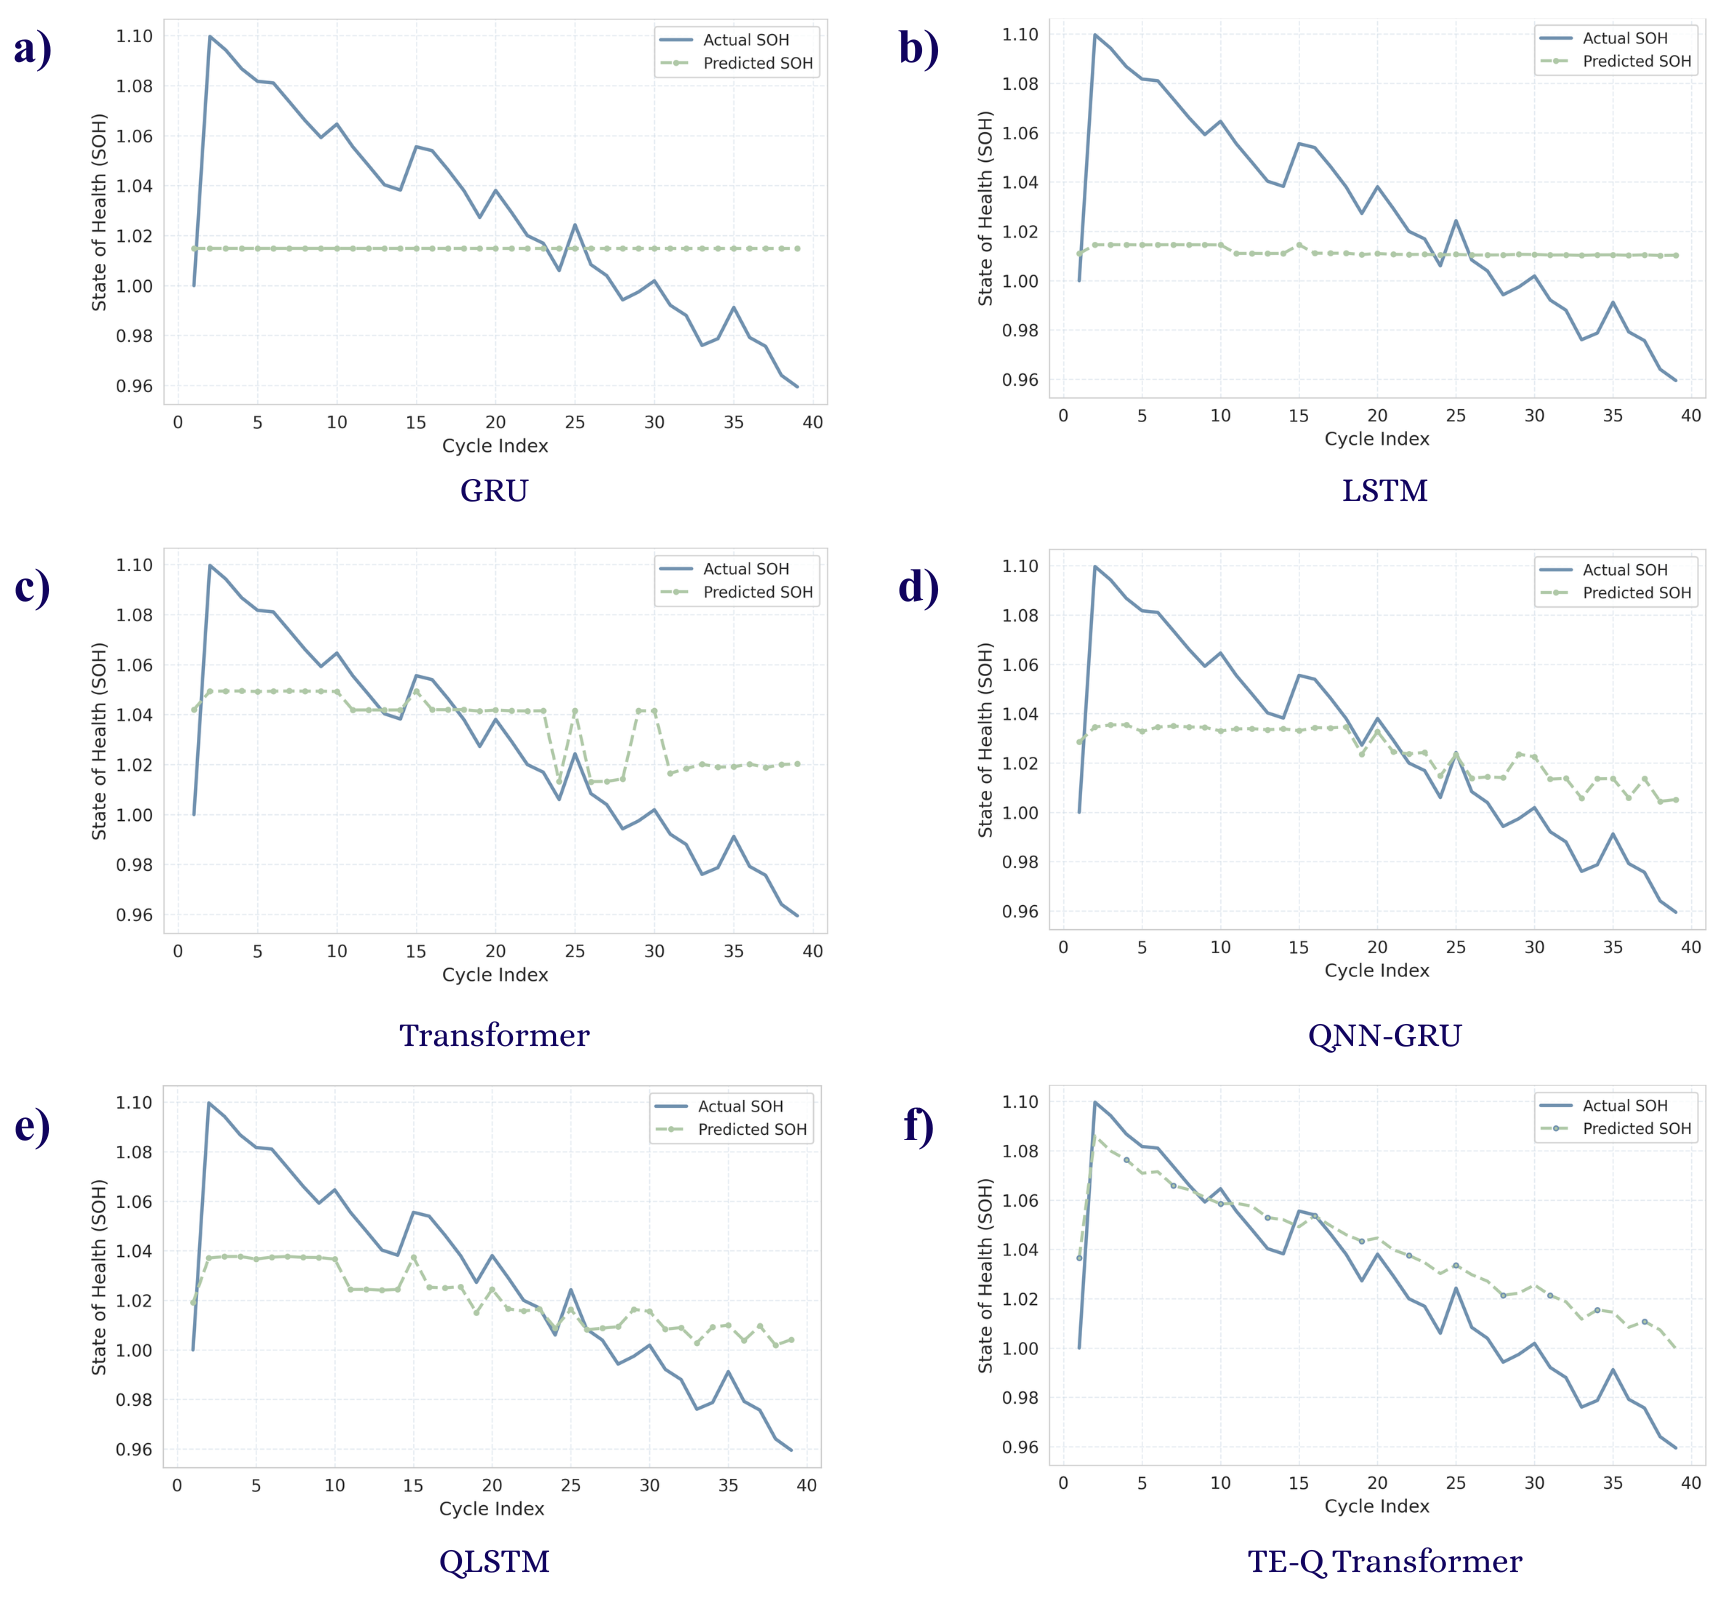
\includegraphics[width=\linewidth]{figs/NASA-b0032.png}
    \caption{Predicted versus actual SOH trajectories for held-out NASA test cell B0032 (43\,$^\circ$C). The TE-Q-Transformer tracks the steep mid-life capacity drop more closely than the baselines.}\label{fig4}
\end{figure}

Figure~\ref{fig2} presents the late-cycle test results for held-out cell B0053 at 4$^\circ$C. Unlike the previous cells, the actual SOH shows short-cycle capacity recovery and therefore does not follow a smooth decreasing trend. GRU, LSTM, Transformer, and QLSTM generally fail to follow this decline, remaining noticeably above the measured SOH during the later cycles. QNN-GRU (Figure~\ref{fig2}d)) performs better than these baselines in following the overall trend, though it still shows visible deviations from the actual trajectory. The TE-Q-Transformer (Figure~\ref{fig2}f)), by comparison, closely tracks both the overall degradation and several local changes, especially in the middle and later portions of the test segment, achieving the lowest RMSE (0.0113) and MAE (0.0095) among all models, together with an $R^2$ of 0.8145. In contrast, the baseline models obtain negative $R^2$ values on this cell, including $-0.5386$ for LSTM, $-1.5595$ for QLSTM, and $-2.9221$ for QNN-GRU. Figure~\ref{fig:nasa_error_boxplot_cells} (right) makes this gap especially clear for the held-out late-life tail: all five baselines shift below zero (consistent overprediction), whereas TE-Q-Transformer stays narrow and near the zero-error line. These results indicate that the TE-Q-Transformer provides a substantially better fit to the complex degradation behavior of B0053.

\begin{figure}%[]
  \centering
    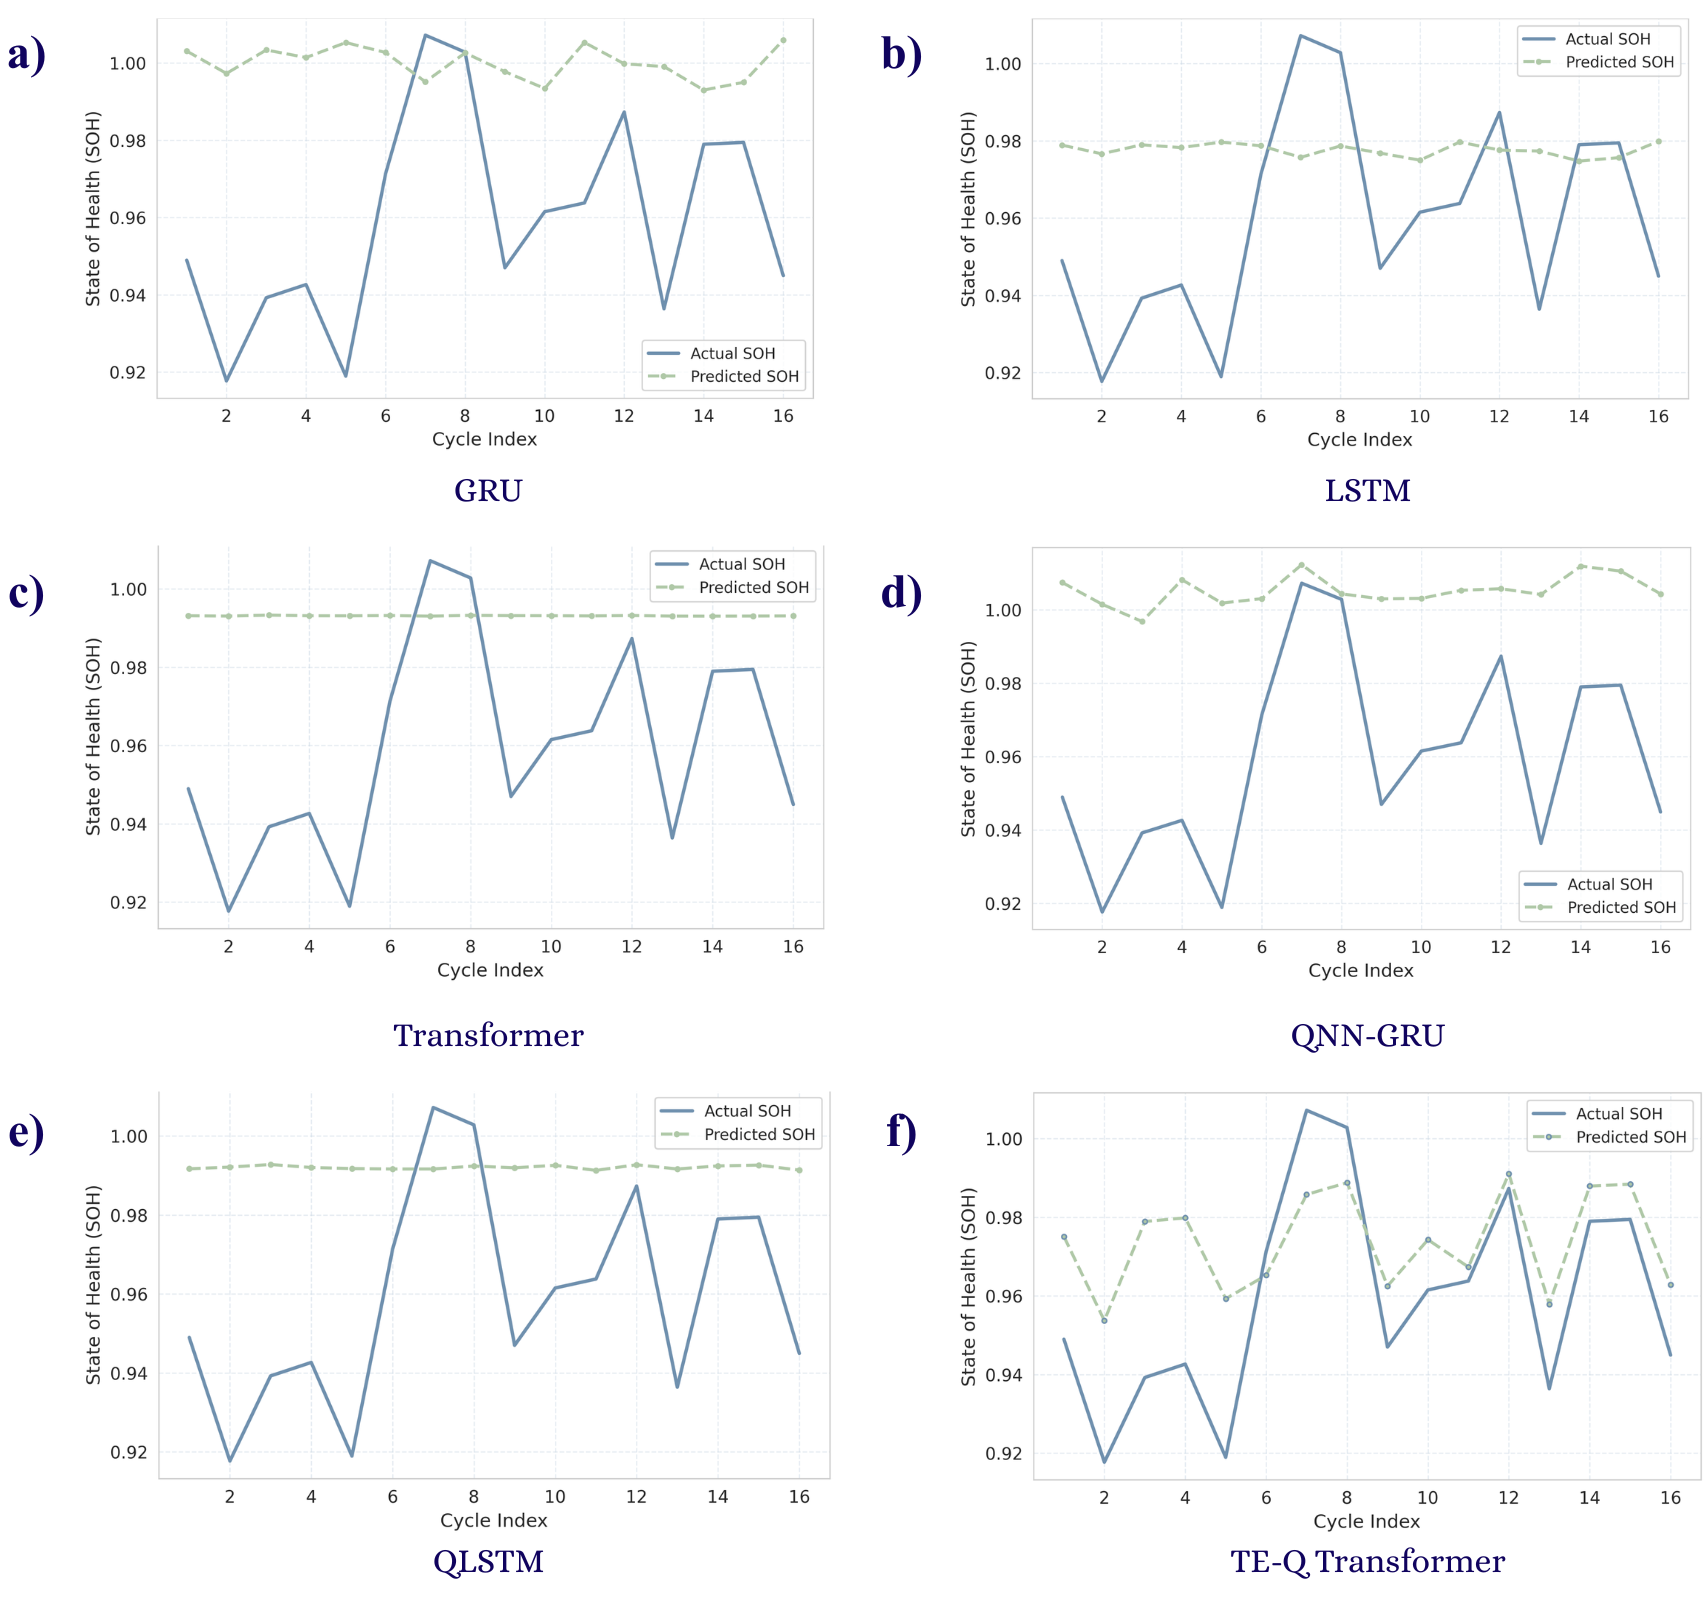
\includegraphics[width=\linewidth]{figs/NASA b0053.png}
    \caption{Predicted versus actual SOH trajectories for the held-out late-cycle test segment of NASA B0053 (4\,$^\circ$C). Non-monotonic short-cycle recovery appears in the actual SOH; the TE-Q-Transformer captures these fluctuations more closely than the other models.}\label{fig2}
\end{figure}

\subsection{Ablation study}
\label{sec:ablation}

This section examines the contribution of each main part of TE-Q-Transformer to the held-out NASA result. We keep the full model as the reference and change one part at a time, while the data split, window size, and training setup stay the same as in Section~\ref{sec:training}. Table~\ref{tab:nasa_ablation} reports the average score over B0018, B0032, and the late test portion of B0053. The last column shows how much RMSE increases after each change. Unlike Table~\ref{tbl5}, which combines all test windows, this table gives equal weight to each cell so that one battery cannot dominate the comparison.

\begin{table*}[t]
\centering
\small
\setlength{\tabcolsep}{4pt}
\caption{Results in different configurations and distinct settings including shared backbone (input 4, sequence length 512, 4 qubits, $d_{\mathrm{model}}=64$, 2 heads, 3 layers, FFN 64, and dropout 0). $\Delta$RMSE is the difference of RMSE between our model with each configuration.}
\label{tab:nasa_ablation}
\begin{tabularx}{\textwidth}{@{}l >{\raggedright\arraybackslash}X cccccc@{}}
\toprule
Settings & Configuration & RMSE & MAE & MAPE & $R^2$ & MaxE & $\Delta$RMSE \\
\midrule
Basic entangler & Rich $\rightarrow$ basic & 0.0388 & 0.0320 & 3.53 & 0.342 & 0.0743 & $+0.0221$ \\
Pauli feature map & $+$ Pauli map & 0.0206 & 0.0166 & 1.78 & 0.774 & 0.0603 & $+0.0038$ \\
No temporal conv & $-$ temporal conv & 0.0261 & 0.0231 & 2.50 & 0.618 & 0.0554 & $+0.0093$ \\
GRU smoother & GRU replaces conv & 0.0274 & 0.0217 & 2.38 & 0.649 & 0.0610 & $+0.0107$ \\
No PE & $-$ positional encoding & 0.0330 & 0.0268 & 2.87 & 0.174 & 0.0862 & $+0.0162$ \\
Mean pooling & Mean pool, no CLS & 0.0237 & 0.0190 & 2.02 & 0.565 & 0.0642 & $+0.0069$ \\
Residual MLP & $+$ residual MLP & 0.0255 & 0.0214 & 2.29 & 0.545 & 0.0628 & $+0.0087$ \\
\textbf{Our model} & Rich, PE, conv $k{=}3$, CLS & \textbf{0.0168} & \textbf{0.0141} & \textbf{1.56} & \textbf{0.870} & \textbf{0.0493} & -- \\
\bottomrule
\end{tabularx}
\end{table*}

The full TE-Q-Transformer is the best row in Table~\ref{tab:nasa_ablation}. It uses the richer quantum mixing described in Section~\ref{sec:architecture}, a short smoothing filter, positional encoding, and a CLS token to summarise each window. This setting reaches an RMSE of 0.0168, an MAE of 0.0141, and an $R^2$ of 0.870. Every other row is worse, which means the reported accuracy comes from these parts working together rather than from one module alone.

The largest drop appears when the richer quantum mixing is replaced by a simpler entangler. RMSE rises to 0.0388 and $R^2$ falls from 0.870 to 0.342. In other words, the four qubits need the stronger mixing pattern to turn temperature-aware inputs into useful features for unseen cells. Adding a Pauli feature map on top of the existing embedding has the opposite character: it is the smallest change in the table, with RMSE 0.0206. The extra encoding still does not beat the full model, so a more complex quantum input map is not helpful here.

The short smoothing filter also matters. Removing it raises RMSE to 0.0261 and lowers $R^2$ to 0.618. Putting a GRU in its place is no better (RMSE 0.0274). A light local smoother is therefore enough, because the transformer already looks across the full sequence.

Two sequence choices are equally clear. Without positional encoding, the model largely loses the ageing trend: $R^2$ drops to 0.174, and the largest single error in the table appears (MaxE 0.0862). The transformer needs to know the order of time steps. Replacing the CLS token with simple averaging also weakens the fit ($R^2$ 0.565). Adding an extra residual MLP after the smoother likewise increases error (RMSE 0.0255). More classical layers do not make up for the parts already in the design.

Overall, Table~\ref{tab:nasa_ablation} points to the same conclusion. The richer quantum mixing and positional encoding matter most, followed by the local smoother and the CLS token. Extra add-ons, including a Pauli map, a GRU smoother, and a residual MLP, do not improve the full model. The proposed setting is therefore the simplest combination that stays accurate on the three held-out temperature conditions.

\subsection{Evidence-based analysis of key claims}\label{sec:discussion}

The discussion below addresses the main claims of this study.

The claim of best point-wise accuracy is supported by RMSE of 0.0312 and MAE of 0.0257 for TE-Q-Transformer, both lower than the five baselines in Table~\ref{tbl5}. QNN-GRU is the closest competitor with RMSE (0.0339), but the proposed model still achieves lower error at the window level on the combined held-out test split. This is consistent with the conclusion that the TE-Q-Transformer pipeline is a better average predictor under the hybrid cross cell protocol.

The claim that TE-Q-Transformer is the only model with positive R\textsuperscript{2} is based on a value of 0.5164, indicating that the model accounts for some of the variation in SOH beyond the constant mean prediction. No baseline attains this: LSTM is very low (0.0010), GRU, Transformer, QNN-GRU and QLSTM all result in negative values. The differences between TE-Q-Transformer and the other models are thus evident with respect to point error, overall fit, and not just RMSE or MAE.

The cross-cell generalization claim follows from the test split in Section~\ref{sec:training}, where we split training from testing based on cell identity, and in the case of B0053 based on cycle order. B0018 and B0032 never appear in training, and the three test conditions span 4\,$^\circ$C, 24\,$^\circ$C, and 43\,$^\circ$C. Strong performance on this split therefore reflects generalization to unseen cells and temperatures rather than performance on randomly mixed cycles from the same cells.

The slow capacity loss as illustrated in Figure~\ref{fig3} in the long cycle range at room temperature is presented for B0018. The general downward trend is captured by TE-Q-Transformer but LSTM can be seen to produce a curve that is nearly flat. This pattern is helpful to understand why the R\textsuperscript{2} value of LSTM approaches 0, and how the proposed model does better in revealing the gain along a full held out trajectory.

As can be seen in Figure~\ref{fig4}, the SOH loss is sharper at 43\,$^\circ$C for the steep mid-life drop of B0032 than the baselines, which tend to lag or smooth the drop. For B0032, the drop in SOH is sharper at 43\,$^\circ$C than that of the baselines. This case is an instance of generalization in a high temperature ageing to a pattern that was not fully trained as a cell.

For short-cycle recovery on B0053, the late-cycle segment at 4\,$^\circ$C in Figure~\ref{fig2} shows short-term SOH recovery rather than steady fade. TE-Q-Transformer follows these fluctuations more closely than the other models. This is the most variable of the three test conditions and shows that the model can respond to low-temperature, non-linear behavior rather than only to smooth degradation.

The claim that classical baselines are weak on R\textsuperscript{2} is supported by GRU ($-$0.6906), Transformer ($-$0.3277), and LSTM (0.0010), all at or below a mean SOH predictor despite sharing the same inputs and protocol. Their qualitative plots also show smoothing or flat outputs, especially for LSTM on B0018. These results suggest that standard sequence models alone do not generalize well under strict cross-cell evaluation on the NASA split used here.

The claim on hybrid QML without thermal physics is supported by QNN-GRU and QLSTM, which include quantum components but still give negative R\textsuperscript{2} values ($-$0.5235 and $-$0.1778). QNN-GRU lowers RMSE relative to some classical models, yet it remains below the mean baseline on R\textsuperscript{2}. Quantum layers alone therefore do not appear sufficient when temperature is not encoded through explicit ageing physics.

The ablation in Section~\ref{sec:ablation} supports this view. The full model needs its richer quantum mixing, position information, local smoothing, and CLS token together. Adding extra layers on top of the same design does not improve accuracy.

Together, these findings point to a consistent pattern. The Arrhenius-informed quantum embedding maps raw temperature to rotation angles through trainable SEI and lithium-plating terms before the Transformer stage. That design aligns with the cross-temperature gains on B0018, B0032, and B0053 and with the clear separation from baselines in Table~\ref{tbl5}. Further work on more datasets and field data is still needed, but on the NASA benchmark studied here, embedding thermal effects in the quantum stage appears to support more reliable cross-cell SOH estimation than classical or hybrid models that treat temperature as an ordinary input.

\noindent\fbox{%
\parbox{\dimexpr\linewidth-2\fboxsep-2\fboxrule\relax}{%
\textbf{Summary:}
On the hybrid multi-temperature held-out split, TE-Q-Transformer delivers the lowest point-wise error (RMSE 0.0312, MAE 0.0257) and is the only model with a positive R\textsuperscript{2} (0.5164), whereas classical and hybrid baselines stay near zero or negative.
These gains appear on fully unseen cells and temperatures: gradual fade at 24\,$^\circ$C (B0018), a steep mid-life drop at 43\,$^\circ$C (B0032), and short-cycle recovery at 4\,$^\circ$C (late B0053).
Hybrid quantum baselines without Arrhenius thermal encoding do not reach the same fit, which supports embedding temperature-driven ageing physics in the quantum stage as a material factor in the cross-cell improvement.
}}

\subsection{Cross-dataset validation on CALCE}\label{sec:calce}

The results above come from the NASA benchmark alone. To check whether the Arrhenius-informed design also holds on a different laboratory, chemistry, and cycling protocol, we repeat the same six models, the same 512-step windowing, and the same cross-cell held-out logic on the CALCE dataset described in Section~\ref{sec:datasets}. Table~\ref{tbl:calce} reports RMSE, MAE, and R\textsuperscript{2} on the combined CALCE test split, which pools the fully held-out cell CS2\_38 with the chronologically held-out late 30\% of CS2\_37.

\begin{table}%[]
\caption{Model performance on the CALCE dataset. Lower RMSE and MAE, and higher R\textsuperscript{2} are better.}\label{tbl:calce}
\begin{tabular*}{\tblwidth}{@{}LLLL@{}}
\toprule
Model & RMSE & MAE & R\textsuperscript{2} \\
\midrule
Wang et al.~\citep{wang2024state} (GRU) & 0.0504 & 0.0421 & 0.8050 \\
Zhang et al.~\citep{zhang2023accurate} (LSTM) & 0.0447 & 0.0356 & 0.8417 \\
Giuliano et al.~\citep{giuliano2025transformer} (Transformer) & 0.0736 & 0.0659 & 0.5516 \\
Soon and Soon \citep{soon2025hybrid} (QNN-GRU) & 0.0478 & 0.0344 & 0.8270 \\
Wang and Kebede \citep{wang2026prediction} (QLSTM) & 0.0517 & 0.0361 & 0.7963 \\
Proposed (TE-Q-Transformer) & \textbf{0.0409} & \textbf{0.0334} & \textbf{0.8704} \\
\bottomrule
\end{tabular*}
\end{table}

Unlike the NASA split, every model reaches a positive R\textsuperscript{2} on CALCE, which reflects the more regular, single-temperature cycling protocol of the CS2 cells. Even so, TE-Q-Transformer remains the best model on all three metrics: it obtains the lowest RMSE (0.0409) and MAE (0.0334) and the highest R\textsuperscript{2} (0.8704) among the six models. The Transformer baseline is clearly the weakest model on CALCE (RMSE 0.0736, R\textsuperscript{2} 0.5516), while LSTM is the strongest of the five baselines (RMSE 0.0447, R\textsuperscript{2} 0.8417). The two quantum-classical baselines, QNN-GRU and QLSTM, sit between GRU and LSTM on R\textsuperscript{2} but do not close the gap to the proposed model, which suggests that adding a generic quantum layer without an explicit thermal mechanism is again not enough to match TE-Q-Transformer, consistent with the NASA findings in Section~\ref{sec:results}.

\begin{figure}%[]
  \centering
    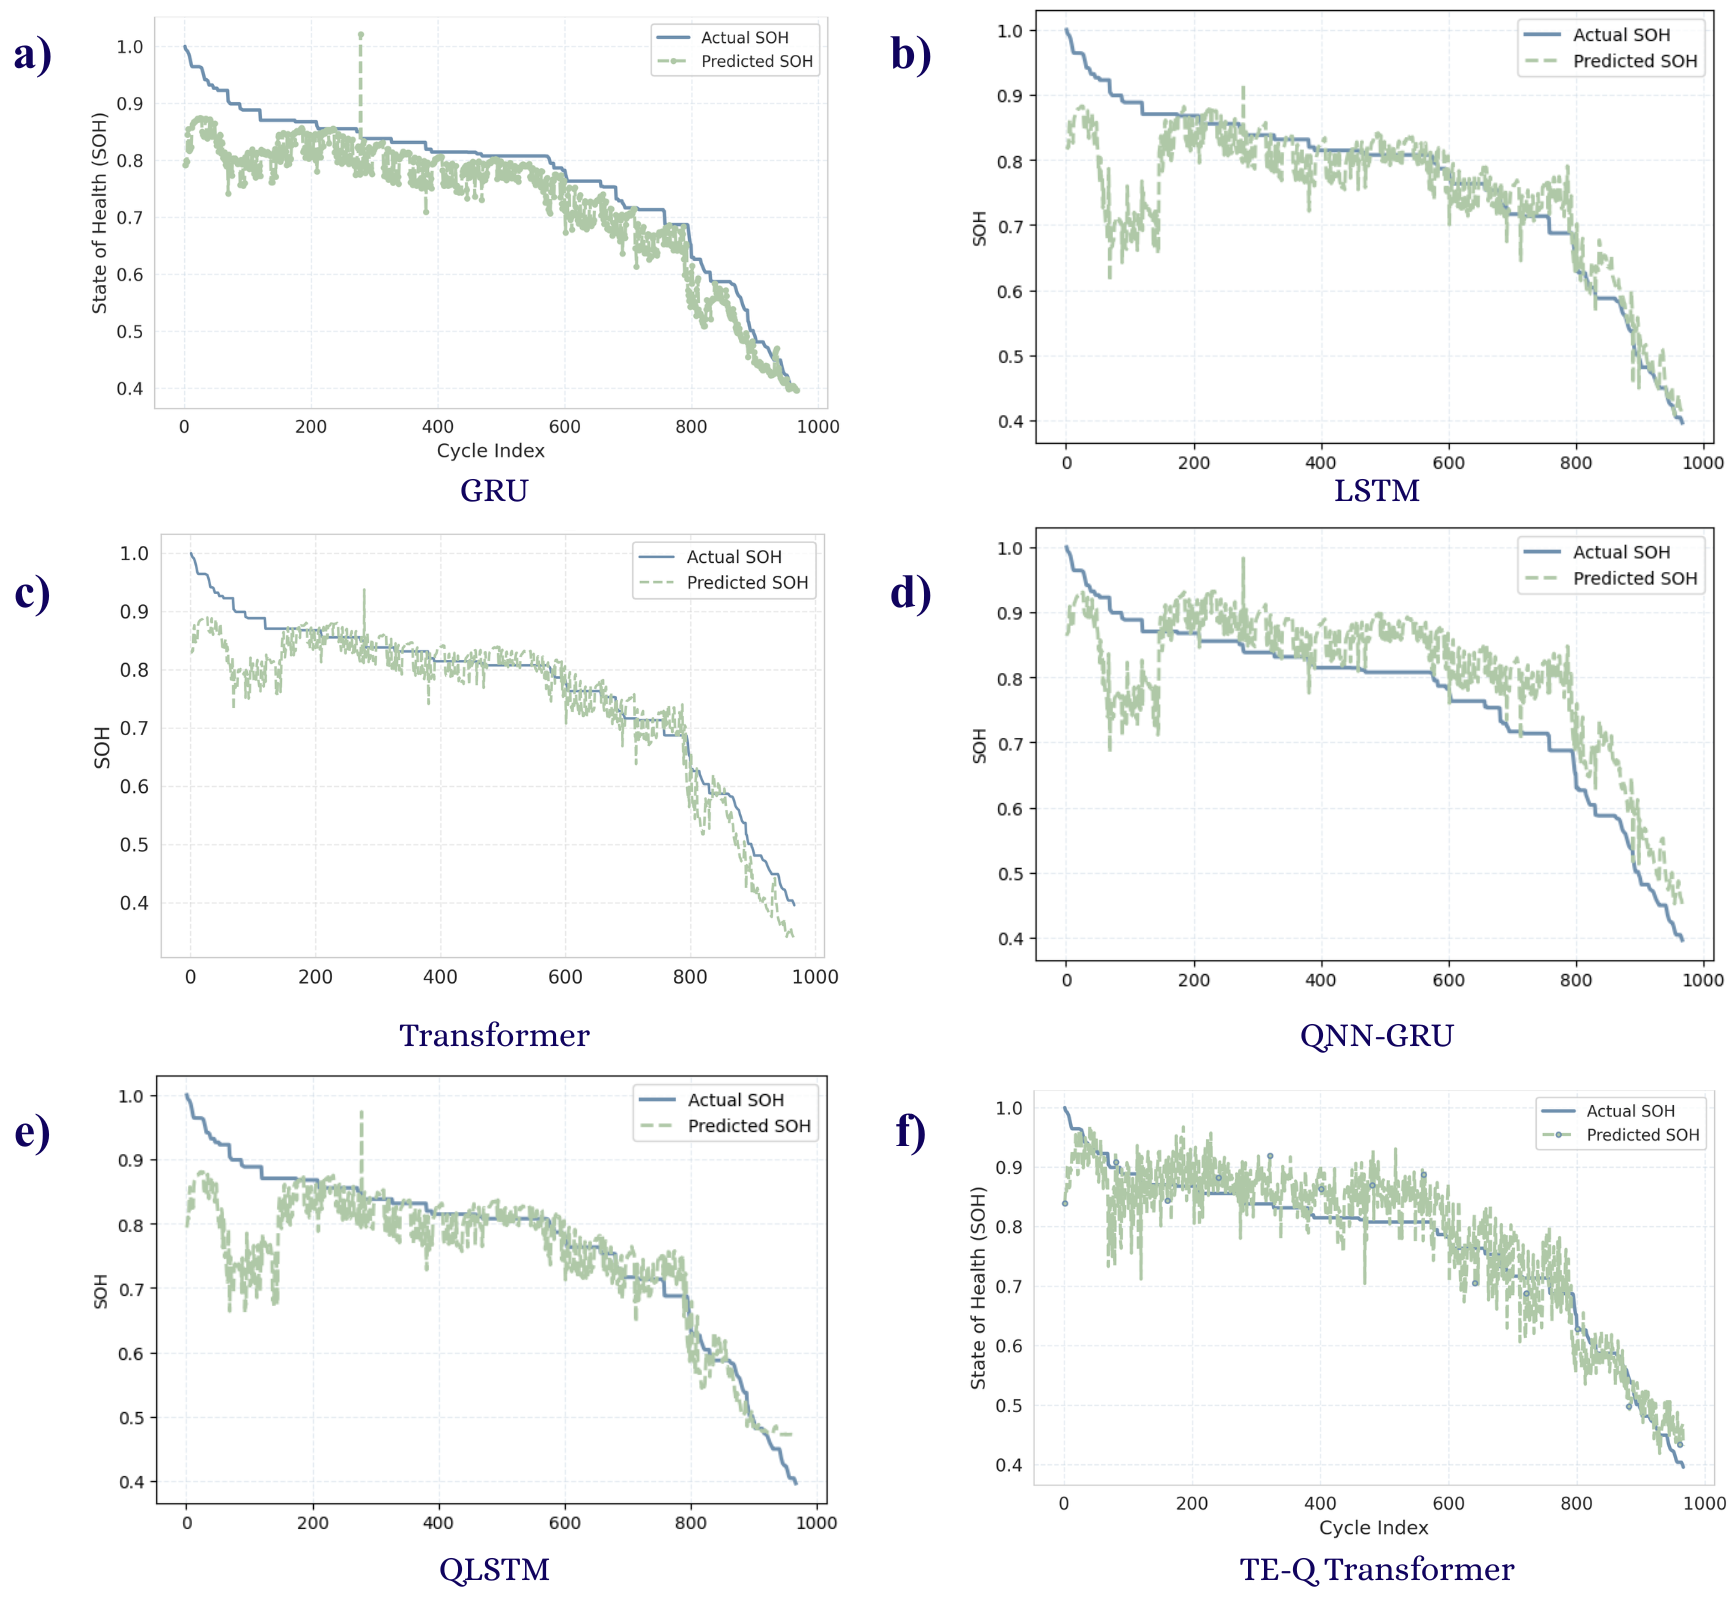
\includegraphics[width=\linewidth]{figs/CALCE CS2-38.png}
    \caption{Predicted versus actual SOH trajectories for the fully held-out CALCE test cell CS2\_38. TE-Q-Transformer (f) tracks the degradation curve more closely than the five baselines, which show larger early-cycle deviations and a noisier fit around the mid-life region.}\label{fig:calce38}
\end{figure}

Figure~\ref{fig:calce38} shows the full predicted-versus-actual trajectory for CS2\_38. GRU, LSTM, Transformer, and QLSTM all show a noisy early-to-mid life segment, where the predicted SOH swings well below and, for LSTM, Transformer, and QLSTM, then well above the actual curve before settling closer to the true trend after roughly cycle 200. QNN-GRU shows a similar early dip and then overshoots the actual SOH for most of the middle portion of the trajectory. TE-Q-Transformer follows the initial decline more smoothly and stays closer to the actual curve for most of the cell's life, with the largest visible deviations appearing in the final cycles, where the true SOH falls sharply.

\begin{figure}%[]
  \centering
    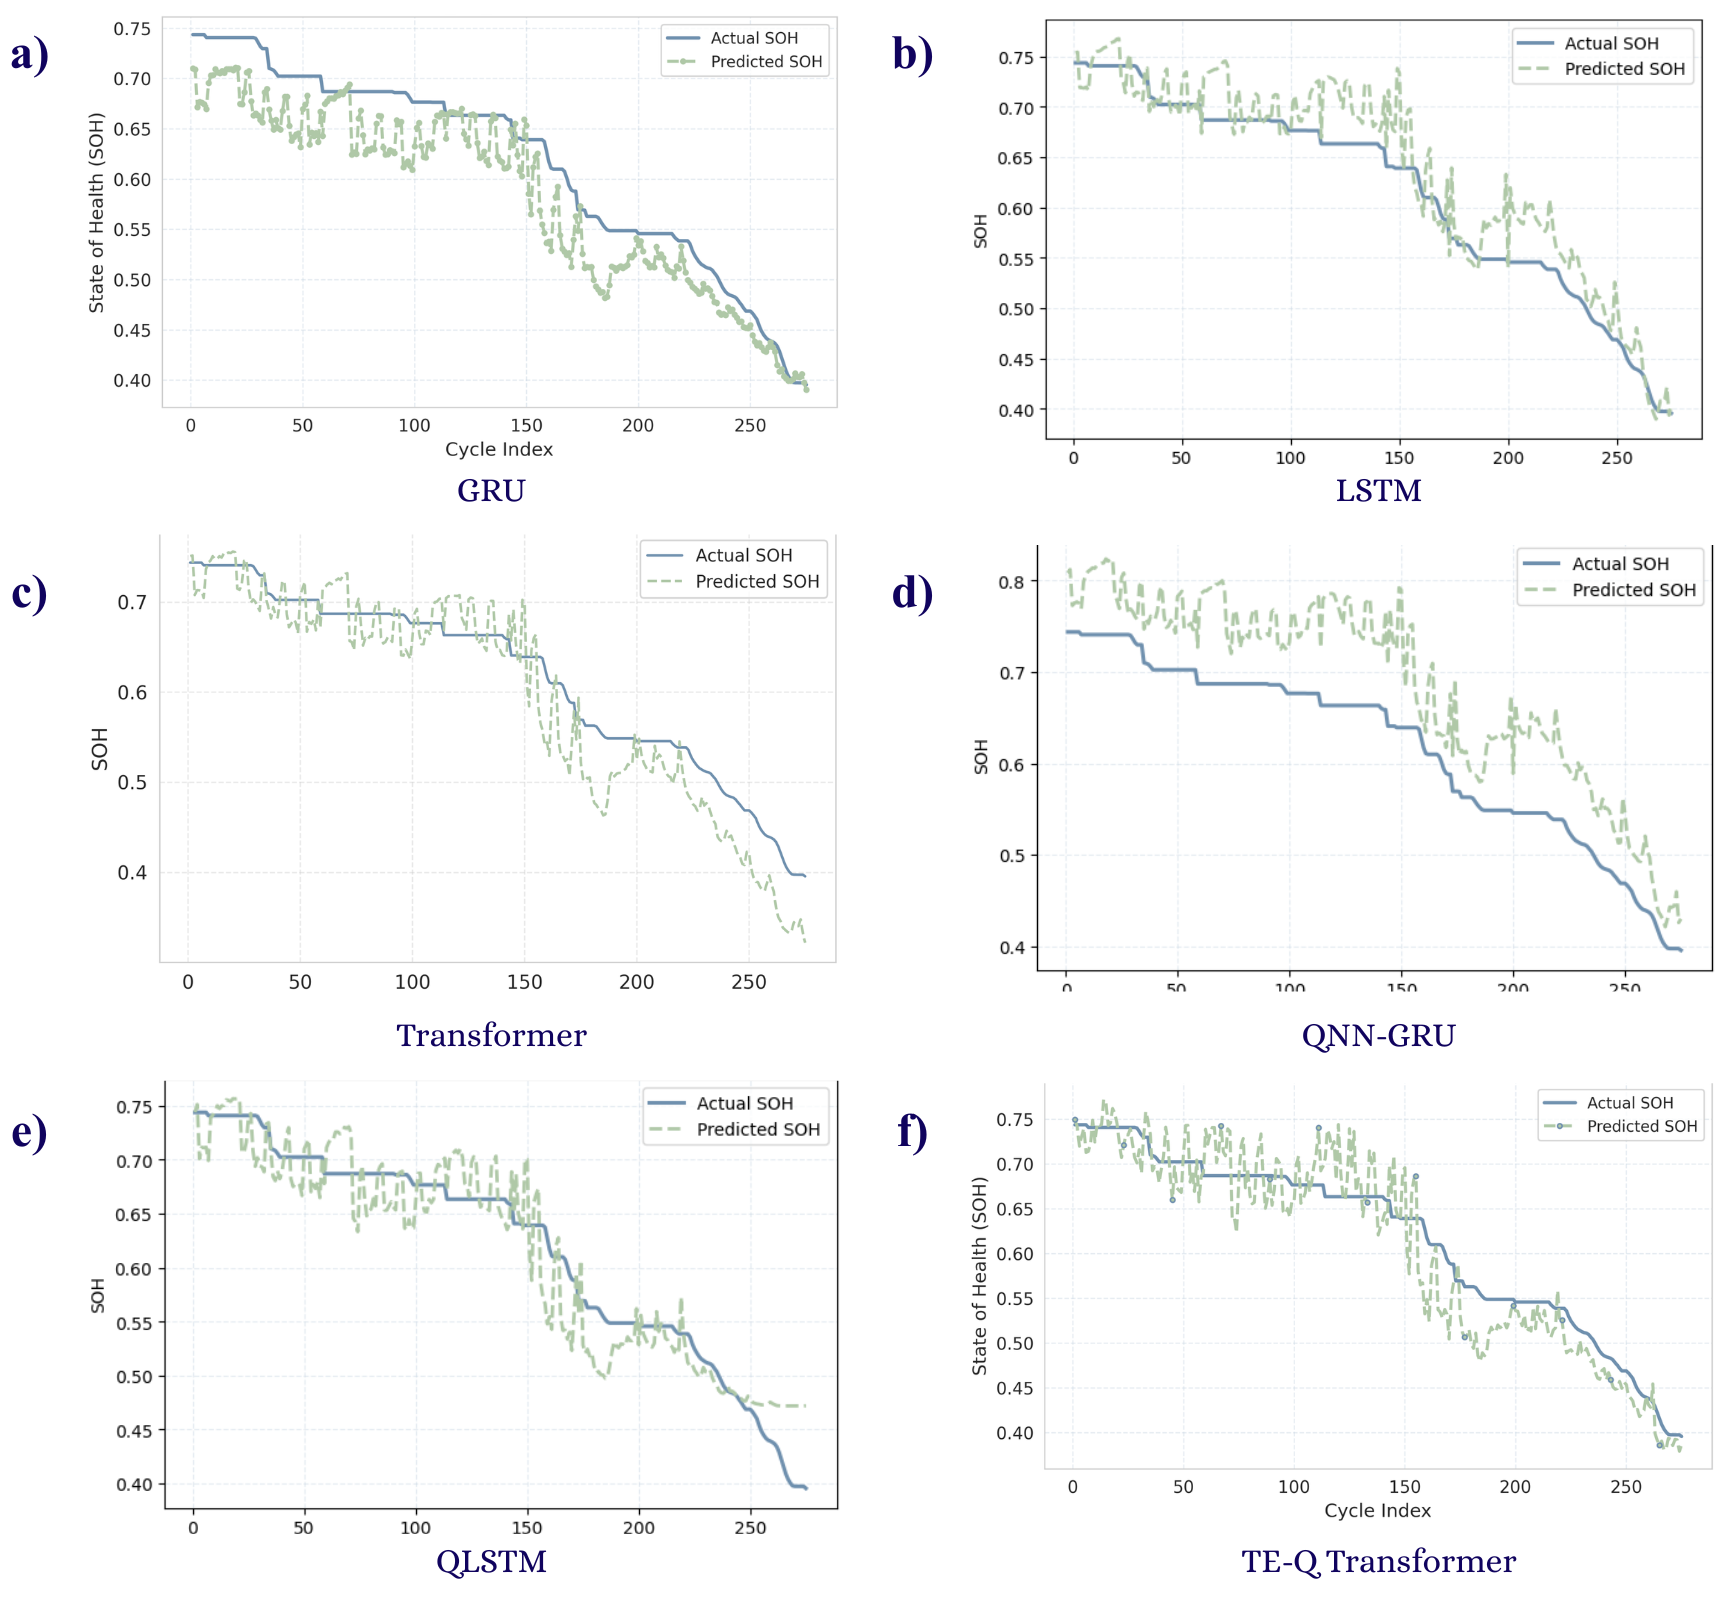
\includegraphics[width=\linewidth]{figs/CALCE CS2-37.png}
    \caption{Predicted versus actual SOH trajectories for the held-out late-cycle test segment of CALCE cell CS2\_37. The TE-Q-Transformer tracks the mid-life plateau and the late-cycle decline with fewer large excursions than the baseline models.}\label{fig:calce37}
\end{figure}

Figure~\ref{fig:calce37} shows the corresponding late test segment of CS2\_37, the CALCE analogue of the B0053 held-out tail on NASA. GRU, LSTM, Transformer, and QLSTM again track the general downward trend but oscillate visibly around it, particularly during the flatter region between roughly cycle 50 and cycle 150. QNN-GRU is the least stable model on this cell, with predictions that repeatedly overshoot the actual SOH by a wide margin in the same region. TE-Q-Transformer stays closer to the actual curve through both the plateau and the steep decline after cycle 250, mirroring the pattern already observed on the NASA cells in Section~\ref{sec:qualitative}.

Taken together with Table~\ref{tbl:calce}, these two trajectories indicate that the gains from the Arrhenius-informed quantum embedding are not specific to the NASA cells or their wider temperature range. The same architecture, trained under the same protocol, keeps its ranking as the best of the six models on a separate dataset with a different chemistry and a single fixed cycling temperature.

% \clearpage


% \section{Threats to validity}\label{sec:threats}

% \subsection{External validity}
% The empirical findings are limited to the NASA PCoE and CALCE laboratory cells used in this study. The training and test cells within each dataset share a common experimental setting, and while CALCE gives a second chemistry and test bench, both datasets are still small-format laboratory cells cycled under controlled conditions.
% % and do not cover pack-level behaviour, field duty cycles, or other open datasets. 
% Ambient temperatures on the NASA held-out set span 4\,$^\circ$C, 24\,$^\circ$C, and 43\,$^\circ$C, which supports a multi-temperature check but is still a sparse sample of real operating conditions; the CALCE cells, by contrast, are cycled at a single fixed temperature, so the CALCE result checks cross-chemistry generalization rather than the temperature range itself. Performance may therefore change under different chemistries, sampling rates, or vehicle-level data. 
% The quantum part of the proposed architecture is also simulated in PennyLane rather than executed on physical quantum hardware.
% % so reported gains should be read as evidence for the hybrid classical-simulation pipeline, not as a claim about near-term quantum devices.
% In addition, the component ablation in Section~\ref{sec:ablation} was carried out on NASA only; we have not verified that every part of the design contributes in the same way on CALCE, so the CALCE result in Section~\ref{sec:calce} should be read as evidence for the full model rather than for each of its components individually.

% \subsection{Internal validity}
% We use a single fixed hybrid multi-temperature cross-cell held-out split rather than $k$-fold or leave-one-battery-out rotation. That choice reduces optimistic leakage from mixing cycles of the same cell across train and test.
% % , but it also means the metrics depend on this particular partition. 
% In particular, B0018 and B0032 are fully held out, whereas B0053 contributes early cycles to training and only its late 30\% to testing, so cold-temperature behaviour is not completely unseen. The CALCE split follows the same rule: CS2\_38 is fully held out, while CS2\_37 contributes its first 70\% of cycles to training and only its late 30\% to testing.
% % All models share the same 512-step windows, train-only min-max scaling for voltage, current, and time, and raw Celsius temperature for the Arrhenius gate. 
% % This equalizes the protocol, yet hyperparameter choices, training schedules, and our re-implementations of GRU, LSTM, Transformer, QNN-GRU, and QLSTM may still differ from the original papers that motivated those baselines. Residual differences in optimization or capacity could therefore contribute to the observed gaps alongside the proposed architecture.

% \subsection{Construct validity}
% SOH is defined as current measured capacity divided by each cell's first-cycle capacity. This is a standard laboratory construct. However, it does not capture impedance growth, power fade, or pack-level state of health used in some BMS settings. 
% % The Arrhenius gate encodes temperature through trainable SEI and lithium-plating activation energies that shape rotation angles; those parameters are learned from data and are not constrained to measured physical constants, so the gate is physics-informed rather than a calibrated ageing model. 
% Input windows use voltage, current, temperature, and normalized time only. Complementary health indicators such as incremental capacity features or impedance spectra are outside the present construct. 

% % Finally, RMSE, MAE, and R\textsuperscript{2} on window-level predictions summarize point error and fit on the combined test split; they do not alone certify cycle-life prognosis or safety-critical deployment readiness.

\section{Conclusion}
\label{sec:conclusion}
Reliable battery health monitoring is essential for ensuring the safety, performance, and longevity of lithium-ion battery-powered systems. Existing data-driven SOH estimation models do not adequately capture the effects of temperature on battery degradation, which limits their performance on unseen lithium-ion battery cells under different temperature conditions.
This work presents TE-Q-Transformer, a hybrid quantum-classical framework for lithium-ion battery SOH estimation that embeds Arrhenius-based thermal ageing into a four-qubit feature circuit before a compact transformer encoder. Here, temperature is mapped through trainable SEI and lithium-plating activation energies rather than treated as an ordinary scaled input, while voltage, current, and normalized time use $\pi$-scaled rotations. On the NASA dataset under a fixed hybrid multi-temperature cross-cell held-out protocol, TE-Q-Transformer achieved an RMSE of 0.0312, an MAE of 0.0257, and an R\textsuperscript{2} of 0.5164, outperforming five classical and hybrid quantum baselines and remaining the only model with a positive R\textsuperscript{2}. 
The results on held-out cells at 24\,$^\circ$C, 43\,$^\circ$C, and 4\,$^\circ$C further show closer tracking of gradual fade, steep mid-life drop, and short-cycle recovery. 
On the independent CALCE dataset, using the same cross-cell held-out protocol and the same six models, TE-Q-Transformer again gave the best result, with an RMSE of 0.0409, an MAE of 0.0334, and an R\textsuperscript{2} of 0.8704, ahead of GRU, LSTM, Transformer, QNN-GRU, and QLSTM.
These results indicate that physics-informed temperature encoding in the quantum stage can improve cross-cell SOH estimation under varying thermal conditions, and that the same architecture generalizes to a second dataset with a different chemistry and cycling protocol. 

Future work will extend the evaluation to more diverse laboratory and field datasets,including broader temperature ranges and different battery chemistries. Further improvements will explore hardware-efficient quantum circuits, noise-aware training, and more advanced physics-informed mechanisms to enhance scalability, robustness, and cross-battery generalization.

% To print the credit authorship contribution details

\printcredits

\section*{Declaration of generative AI tools use in the writing process}
During the preparation of this manuscript, the authors used ChatGPT to improve the language and readability of the text. The authors reviewed and verified all content and take full responsibility for the final manuscript.
%% Loading bibliography style file
\bibliographystyle{model1-num-names}

% Loading bibliography database
\bibliography{cas-refs}

% Biography
%\bio{}
% Here goes the biography details.
%\endbio

%\bio{pic1}
% Here goes the biography details.
%\endbio

\end{document}